%% TODO: Summary of the report here (1-2 pages)

\newpage

\begin{abstract}
    Abstract
\end{abstract}

\maketitle

\subsubsection*{Acknowledgements:}

\section{Introduction}\label{sec:introduction}
NASA has been studying the Martian environment for decades through a series of missions, including the Viking missions~\cite{marsnasagov_vikings}, the \gls{mer} mission~\cite{marsnasagov_observer, marsnasagov_spirit_opportunity}, and the \gls{msl} mission~\cite{marsnasagov_msl}, each building on the knowledge gained from the previous ones.
Today, the rovers exploring Mars are equipped with sophisticated instruments for analyzing the chemical composition of Martian soil in search of past life and habitable environments.

Part of this research is facilitated through interpretation of spectral data gathered by \gls{libs} instruments, which fire a high-powered laser at soil samples to create a plasma.
The emitted light is captured by spectrometers and analyzed using machine learning models to assess the presence and concentration of certain major oxides, informing NASA's understanding of Mars' geology~\cite{cleggRecalibrationMarsScience2017}.

However, predicting major oxide compositions from \gls{libs} data still presents significant computational challenges.
These include the high dimensionality and non-linearity of the data, compounded by issues of multicollinearity and matrix effects~\cite{andersonImprovedAccuracyQuantitative2017}.
Such effects can cause the intensity of emission lines from an element to vary independently of that element's concentration, introducing unknown variables that complicate the analysis.
Furthermore, the high cost of data collection often results in small datasets, exacerbating the difficulty of building accurate and robust models.

Previous work has aimed to improve the prediction of major oxide compositions from \gls{libs} data by using regression techniques and dimensionality reduction with feature selection.
These methods have been used to enhance both the accuracy and interpretability of the prediction models.
Tailored approaches have also been developed, where different models are selected based on their performance with specific spectral characteristics~\cite{rezaei_dimensionality_reduction, andersonPostlandingMajorElement2022}.
Moreover, models incorporating physical principles have demonstrated improved accuracy by handling residuals that traditional models fail to explain~\cite{song_DF-K-ELM}.
However, predicting oxide compositions remains challenging due to the complex, nonlinear nature of \gls{libs} data.
This underscores the need for continued research into more adaptive and robust machine learning strategies to tackle these issues effectively.

This thesis aims to improve upon previous work in the field of \gls{libs} data analysis.
Our goal is to develop a machine learning pipeline that is tailored to the unique characteristics of \gls{libs} data, with the goal of achieving higher prediction accuracy and robustness.

To achieve these objectives, we build upon the baseline established in~\cite{p9_paper} and systematically explore ten different machine learning models. 
These models were identified and selected through a combination of extensive literature review and the consideration of unconventional approaches not typically covered in the \gls{libs}-based calibration literature.
The ten models fall into three categories: Ensemble learning models, linear and regularization models, and neural network models.
In addition to model exploration, we also investigate a selection of preprocessing techniques: scaling (including normalization), dimensionality reduction, and data transformation.
Specifically, we designed and implemented a framework for experimental analysis using the automated hyperparameter optimization framework Optuna~\cite{optuna_2019}.
We then used this framework to determine the most effective combinations of preprocessing methods and models for each regression target.
We began by identifying the most promising models from the literature, after which we evaluated various preprocessing techniques to understand their impact on model performance, selecting those that demonstrated the highest impact on improving the performance of each model.
Following preprocessing, we optimized the chosen models through hyperparameter tuning to ensure optimal performance tailored to the specific data characteristics of each oxide.
Once the best hyperparameters were identified, a stacking ensemble method was employed to create a meta learner for each oxide, significantly enhancing prediction accuracy and robustness beyond the capabilities of individual models.
% TODO: Superior performance needs to be replaced with actual numbers
Through extensive experiments on \gls{libs} data, we systematically assessed and demonstrated the superior performance of our approach compared to existing methods, focusing on significant improvements in prediction accuracy and robustness.

Our key contributions are as follows:
\begin{itemize}
    \item We develop a novel machine learning pipeline that demonstrates improved accuracy and robustness in predicting major oxide compositions in \gls{libs} data.
    \item We have developed a novel optimization approach and tool for tuning and evaluating machine learning models along with preprocessing techniques, providing a systematic and efficient method for selecting the best configuration.
    \item By outperforming existing methods, our approach has established new benchmarks for accuracy and robustness in \gls{libs} data analysis.
\end{itemize}


% TODO: Add remaining sections
The remainder of this paper is organized as follows:
Section~\ref{sec:background} provides background on the onoging Mars exploration missions, the \gls{libs} technique, and the baseline \gls{moc} model.
Section~\ref{sec:problem_definition} formally defines the problem addressed in this work.
Section~\ref{sec:methodology} describes our proposed methodology, including data preprocessing, dimensionality reduction, and machine learning models.
Section~\ref{sec:experiments} presents our experimental setup and results.
Finally, Section~\ref{sec:conclusion} concludes the paper and discusses future work.

In table \ref{tab:terms}, we provide a list of terms used throughout this paper.

\begin{table}
\centering
\begin{tabularx}{\columnwidth}{lX} % l for left, X for the cell that should be wrapped
\toprule
Term & Definition \\
\midrule
Sample & A physical specimen of rock, soil, or other material collected for scientific analysis.\\
Location & The specific point on a sample where a LIBS laser is targeted. There are typically multiple locations per sample. \\ 
Target & Refers to the variable that a machine learning model is trained to predict. \\
\bottomrule
\end{tabularx}  
\caption{Table of Terms}
\label{tab:terms}
\end{table}
\section{Related Work}
In addressing the challenge of predicting major oxide compositions from \gls{libs} data, our investigation intersects with a broad spectrum of existing research that tackles similar computational hurdles, such as high dimensionality, multicollinearity, matrix effects, and the challenges of small datasets.
This section outlines how prior works relate to our problem, drawing from a range of techniques and methodologies that offer potential pathways for enhancing the accuracy and robustness of our predictions.

\citet{andersonPostlandingMajorElement2022} experimented with different machine learning models for quantifying major oxides on Mars using the SuperCam instrument on the Mars 2020 Perseverance rover.
They discuss preprocessing, normalization of \gls{libs} spectra, and the development of multivariate regression models to predict major element compositions.
For each oxide, they tested different models and selected the best performing one.
In some cases, they used a blend of models to improve the predictions.
The models they tested include: \gls{ols}, \gls{pls}, \gls{lasso}, Ridge, \gls{enet}, \gls{omp}, \gls{svr}, \gls{rf}, \gls{gbr}, and local \gls{enet} and blended submodels.
For \ce{SiO2}, they used a blend of \gls{gbr} and \gls{pls} models.
Interestingly, they found that PLS performed better at longer distances (4.25m), but GBR was better at 3m.
For \ce{TiO2}, they selected the \gls{rf} model for its superior performance at 4.25m and overall lower \gls{rmsep}.
For \ce{Al2O3}, they used an average of predictions from four models (Local \gls{enet}, \gls{rf}, two variants of \gls{pls}) to obtain the lowest \gls{rmsep}.
For \ce{FeO_T}, they initially selected \gls{rf} but later replaced it with \gls{gbr} due to its more realistic stoichiometry predictions for high-\ce{Ca} pyroxenes and overall performance.
For \ce{MgO}, they selected \gls{gbr} for having the lowest \gls{rmsep} and avoiding negative predictions, despite slightly overpredicting \ce{MgO} for high concentration samples.
For \ce{CaO}, they used a blend of \gls{rf} and \gls{pls} to address the bimodal distribution of \ce{CaO} predictions by the \gls{rf} model alone.
For \ce{Na2O}, they used a blend of \gls{gbr} and \gls{lasso} models to utilize \gls{gbr}'s accuracy at low concentrations and \gls{lasso}'s superior predictions at higher concentrations.
For \ce{K2O}, they selected \gls{lasso} for its better performance on high \ce{K2O} samples, despite the averaged model of five algorithms showing slight improvements at lower concentrations.
The findings of this paper are significant to us because they provide a benchmark for the performance of different machine learning models on \gls{libs} spectra.
We can use this information to guide our model selection and to compare our results with theirs.
Additionally, we might want to try out different models from the ones they tested to see if we can improve the predictions further, or perhaps find a model that is more suitable for our specific use case.
Also, SuperCam being the successor to \gls{chemcam} means that the findings of this paper are directly relevant to our work.

\citet{song_DF-K-ELM} present a novel approach to enhance the performance and interpretability of machine learning models in the context of \gls{libs} quantification.
The authors use "knowledge-based spectral lines, related to analyte compositions, to construct a linear physical principle based model and adopts \gls{k-elm} to account for the residuals of the linear model."
The method is based on \gls{df} and \gls{k-elm} and is called \gls{df}-\gls{k-elm}.
This method stands out by offering an intuitive explanation of how knowledge-based spectral lines impact prediction results, thereby enhancing model interpretability without compromising model complexity.
DF-\gls{k-elm} was tested across 10 regression tasks based on 3 \gls{libs} datasets, comparing its performance against six baseline methods using \gls{rmsep} as the evaluation metric.
They have 3 coal datasets, and they do regression tasks involving carbon, ash, volatile matter, and heat value analysis.
It achieved the best performance in 4 tasks and the second-best in 2 tasks, demonstrating its efficacy.
Incorporation of domain knowledge not only improved the accuracy of the models but also enhanced their generalizability across different tasks.
The method's design allows for a more interpretable machine learning model that adheres closer to the physical principles underlying \gls{libs} quantification.
The integration of domain knowledge into machine learning models addresses two critical challenges: improving the interpretability of complex models and enhancing their performance by leveraging specific domain insights.
The approach demonstrates a practical application of kernel extreme learning machines combined with domain-specific insights.
This is particularly valuable in fields like spectroscopy, where understanding the relationship between the spectral data and the analyte concentration is vital.
The DF-\gls{k-elm} method showcases how hybrid models can outperform traditional machine learning approaches.
The approach demonstrates a practical application of kernel extreme learning machines combined with domain-specific insights.
This is very relevant to our work considering interpretability is a key requirement for NASA and something they considered when choosing the \gls{pls} model for the \gls{chemcam} instrument.

\citet{rezaei_dimensionality_reduction} explore a variety of statistical and machine learning methods, including \gls{mulr}, \gls{svr}, \gls{ksvr}, and \gls{ann}, alongside their integrations with \gls{pca} to reduce dimensionality and improve model performance.
They use \gls{mse} and \gls{mae} as evaluation metrics to compare the performance of the models.
This paper clearly demonstrates the effectiveness of dimensionality reduction techniques in improving the performance of machine learning models because it compares the performance of many models with and without \gls{pca}: \gls{ann}, \gls{mulr}, \gls{svr}, \gls{ksvr}, \gls{pca}-\gls{ann}, \gls{pca}-\gls{mulr}, \gls{pca}-\gls{svr}, and \gls{pca}-\gls{ksvr}.
For all elements, a variant of \gls{svr} performs the best.
For \ce{Si}, \gls{svr} performs the best.
For \ce{Zn}, \gls{pca}-\gls{svr} performs the best.
For the rest of the elements, \gls{pca}-\gls{ksvr} performs the best.
The superiority of \gls{ksvr} is attributed to the its ability to handle non-linear relationships in the data effectively, especially when combined with \gls{pca}'s capability to compress and simplify the input data by focusing on the most relevant variations.

\citet{yang_laser-induced_2022} present a study on the application of a deep \gls{cnn} for classifying geochemical samples using \gls{libs}, with a particular focus on planetary exploration missions such as China's Tianwen-1 Mars mission.
The authors demonstrate the effectiveness of a deep CNN in classifying geochemical standard samples using \gls{libs} spectra collected at varying distances.
This addresses the challenge of spectral differences induced by distance, showcasing that \gls{cnn} can learn to classify samples without the need for traditional spectral preprocessing or distance correction.
Using a dataset of over 18,000 \gls{libs} spectra from 39 geochemical standard samples, the study compares the \gls{cnn} model's performance against four other machine learning models: \gls{bpnn} \gls{svm}, \gls{lda}, and \gls{logreg}.
The \gls{cnn} model exhibits superior classification accuracy, emphasizing its potential for geochemical sample identification/classification in planetary exploration.
The paper includes a detailed comparative analysis, proving the \gls{cnn} model's superior performance.
With classification accuracies on the validation set for all models exceeding 95\%, the \gls{cnn} model demonstrated the highest overall accuracy.
This was particularly evident as the training set size increased, indicating the model's robustness to varying distances without requiring distance correction.
Statistical analysis further confirmed the \gls{cnn} model's superiority, with higher average Ncorr values compared to other models.
The \gls{cnn} model's ability to accurately classify geochemical samples without preprocessing for distance correction is quite impressive.
This is particularly relevant to our work because we are also working with \gls{libs} spectra collected at varying distances.
The comparative analysis underscores the \gls{cnn} model as a best-fit approach for \gls{libs} data analysis, potentially setting a new standard for future research and applications in the field.

\citet{jeonEffectsFeatureEngineering2024} investigated the effects of feature engineering on the robustness of \gls{libs} for steel classification.
They developed a remote \gls{libs} system to classify six steel types, using various feature-engineering and machine learning algorithms, including \gls{svm} and \gls{fcnn}, to handle different laser energies in test datasets.
They found that using intensity ratios as input data resulted in more robust classification models.
It was better than \gls{pca} and \gls{rf}-based wavelength selection.
The study highlights the importance of selecting appropriate feature engineering methods to improve model robustness, especially under varying measurement conditions.
This is relevant to our project as it demonstrates how feature engineering can enhance the performance and robustness of models for classifying materials based on \gls{libs} data, addressing challenges similar to those we face in predicting major oxide compositions.

The study by \citet{fontanaLaserInducedBreakdown2023}.
explores using \gls{libs} for whole-rock geochemical analysis, specifically for major elements like \ce{Al}, \ce{Ca}, \ce{Fe}, \ce{K}, \ce{Mg}, \ce{Na}, \ce{Si}, and \ce{Ti}.
They averaged \gls{libs} spot analyses over 1-mm spaced transects on drill core intervals, demonstrating strong correlations with lab-based geochemistry for elements like \ce{Si}, \ce{Al}, and \ce{Na}.
Different predictive models were used for each element, such as \gls{pls}, \gls{enet}, \gls{lasso}, and \gls{pcr}, showing varied \gls{rmsecv} values indicating the precision of these models.
This method's relevance to our work lies in its potential for rapid, in-situ geochemical analysis, offering a way to overcome challenges related to high dimensionality and non-linearity in \gls{libs} data.

The paper by \citet{sunMachineLearningTransfer2021} introduces transfer learning to \gls{libs} spectral data analysis for rock classification on Mars, significantly improving model performance.
Previously, models trained on laboratory standards (pellets) struggled with physical matrix effects when applied to natural rock spectra.
Transfer learning, leveraging knowledge from one domain to address related problems in another, was applied to overcome this challenge.
The method showed remarkable improvement in \gls{tas} classification accuracy for both polished and raw rock samples, with rates increasing from 25\% and 33.3\% to 83.3\% respectively using machine learning models to 83.3\% with the transfer learning model.
This demonstrates the effectiveness of transfer learning in addressing the physical matrix effect and enhancing model robustness for rock classification on Mars.

\citet{wangDeterminationElementalComposition2023} discusses an advanced methodology for analyzing stream sediments using remote \gls{libs} combined with a \gls{mdsbpnn} algorithm.
This approach yielded highly accurate quantitative analyses of both major and trace elements, with determination coefficients (R2) for major elements exceeding 0.9996 and for trace elements greater than 0.9837, and \gls{rmse} less than 0.73 (major elements).
The study emphasizes the potential of remote \gls{libs} technology, especially for identifying biominerals in geological samples, highlighting its significance for studying ancient planetary environments.

% We had this one last semester IIRC. Might be good to have again?
\citet{leporeQuantitativePredictionAccuracies2022a} provides an in-depth analysis of the effectiveness of using \gls{libs} for geochemical analysis, focusing on the optimization of calibration datasets through the creation of submodels.
It outlines the methodology for collecting and processing \gls{libs} spectra, the development of multivariate models for predicting geochemical compositions, and compares the predictive accuracies of different submodel strategies.
The study finds that while submodels can improve prediction accuracies under certain conditions, the overall effectiveness is contingent upon having a large and diverse calibration dataset.
The research suggests that the optimal use of \gls{libs} for geochemical analysis requires a balance between the specificity of submodels and the breadth of the calibration dataset to ensure accurate and reliable predictions.

\citet{kepesImprovingLaserinducedBreakdown2022} discusses enhancing \gls{libs} model accuracy using transfer learning between ChemCam and SuperCam instruments.
It proposes a method where ChemCam data transforms to approximate SuperCam spectra, improving \gls{cnn} regression models' performance.
Key methods include data augmentation and fine-tuning of \gls{cnn}s with pre-processed and normalized spectra.
This approach outperforms some existing models for specific oxides, demonstrating transfer learning's potential in \gls{libs} analyses for more accurate quantitative models.

\citet{ferreiraComprehensiveComparisonLinear2022} presents an extensive comparison of various algorithms for quantifying lithium in geological samples, with a focus on both linear and non-linear methods.
The study tested algorithms on spectra acquired from a commercial handheld device and a laboratory prototype, highlighting the challenges in quantifying lithium due to effects like saturation and matrix interference.
The results showed that non-linear methodologies, such as \gls{knn} regression, \gls{svr}, and \gls{ann} regression, generally outperformed linear methods by effectively managing saturation and matrix effects, which are common in geological samples.
This research provides valuable insights for future applications in geological sample analysis and could potentially be generalized for other elements in similar contexts.
The paper's findings are particularly relevant to our project as it demonstrates the effectiveness of non-linear machine learning techniques in handling complex, non-linear relationships in high-dimensional \gls{libs} data, aligning with our research objectives of improving major oxide composition predictions from \gls{libs} data.

The study by \citet{liuComparisonQuantitativeAnalysis2022} explores the use of \gls{marscode} \gls{libs} for quantitative analysis of olivine in a simulated Martian atmosphere, focusing on multivariate analysis methods to address challenges posed by \gls{libs} data, such as high dimensionality and multicollinearity.
The methods evaluated include \gls{ulr}, \gls{mvlr}, \gls{pcr}, \gls{plsr}, ridge regression, \gls{lasso}, \gls{enet}, and \gls{bpnn}.
The findings demonstrate the effectiveness of dimension reduction techniques, especially \gls{plsr}, and nonlinear analysis for improving quantitative analysis accuracy of olivine using \gls{libs} data.
This approach is particularly relevant to our work due to the focus on advanced statistical methods and machine learning algorithms for handling complex, high-dimensional \gls{libs} data, aligning with our objectives of improving accuracy and robustness in predicting major oxide compositions.

\cite{yangConvolutionalNeuralNetwork2022} is a study where a \gls{cnn} model is designed to identify twelve types of rocks using \gls{libs} data from the \gls{marscode} for the Tianwen-1 Mars exploration mission.
The classification performance of the \gls{cnn} is compared with \gls{logreg}, \gls{svm}, and \gls{lda}.
The \gls{cnn} model achieved the highest classification accuracy, demonstrating its efficiency in rock identification with \gls{libs} spectra collected in a simulated Martian environment.
This indicates that \gls{cnn}-supported \gls{libs} classification is a promising analytical technique for planetary exploration missions.

\citet{silvaRobustCalibrationModels2022} introduce clustered regression calibration algorithms for \gls{libs} to address quantification challenges in complex sample matrices or wide concentration ranges, focusing on lithium quantification in geology.
They employ unsupervised clustering to group similar samples before applying a tailored linear calibration model to each cluster.
This approach, tested on lithium in exploration drills, outperforms standard linear models, especially in lower concentration regions, and demonstrates good generalizability to unseen data from different rock veins.
The study highlights the potential of clustered regression methods in improving \gls{libs} quantification accuracy and robustness, particularly valuable in mining environments.
Uses Ridge regression, \gls{pls}, dimensionality reduction with \gls{umap} and then k-means clustering, followed by a local model for each cluster, univariate calibration curves.

\citet{woldPrincipalComponentAnalysis1987} provides an in-depth tutorial on \gls{pca}, a fundamental method in multivariate data analysis used for dimensionality reduction, outlier detection, and uncovering the underlying structure in data sets.
The paper covers the history and development of \gls{pca}, its mathematical foundations, applications across various fields, and detailed instructions for data pre-treatment and \gls{pca} implementation.
It emphasizes \gls{pca}'s utility in simplifying complex data sets, enhancing interpretability, and supporting data analysis through the extraction of principal components that capture the most variance in the data.
This work is particularly relevant to our project as it underscores the importance of \gls{pca} in handling high-dimensional data, which aligns with our objectives of improving the prediction accuracy and interpretability of major oxide compositions from \gls{libs} data by effectively managing multicollinearity and high dimensionality challenges.

\citet{bankAutoencoders2021} details various autoencoder architectures and their applications in machine learning, emphasizing their role in dimensionality reduction, feature learning, and generative models.
It explores regularized, denoising, and variational autoencoders, highlighting their advantages in compressing data into lower-dimensional spaces while retaining essential information for reconstruction.
Autoencoders could significantly enhance our ability to handle the high-dimensional nature of \gls{libs} data.
By compressing spectral data into more manageable representations without losing critical information, we can improve model performance, especially in predicting major oxide compositions, by focusing on the most relevant features extracted from the compressed data representation.
This aligns with our objectives of efficient dimensionality reduction and robust predictive modeling.

In their work \citet{caruana_no_1997}, presents a method called \textit{Multitask learning}, which is a method of learning machine models on several related datasets. 
The motivation for this approach stems from the assumption that utilizing multiple, albeit related, datasets can enhance the model's ability to discern patterns and shapes within the data.
\citet{caruana_no_1997} suggest that leveraging shared representations for model training can enable the model to identify underlying attributes in other data sets, even when this new data is small.
This is interesting to our report as one of the major challenges in analyzing LIBS calibration data for Mars is the scarcity of available data.
This scarcity makes it difficult to construct robust models capable of comprehensively understanding the underlying patterns and physical principles within the data.
Utilizing related LIBS data could help the models first learn the general outline, shape and patterns in the LIBS data, making it easier for it to grasp the deeper patterns in the Mars related data.




\section{Problem Definition}\label{sec:problem_definition}
The objective of this research is to develop and validate a computational methodology to enhance the accuracy and robustness of predicting major oxide compositions from \gls{libs} data.
Such quantification of elements in soil samples from \gls{libs} data presents several significant challenges, including the high dimensionality of spectral data, multicollinearity, matrix effects, and limited data availability.

A fundamental premise of this research posits that by effectively addressing these challenges, the accuracy and robustness of predicting elemental concentrations from \gls{libs} data can be significantly enhanced. This assumption is supported by several key studies in the field.
For instance, \citet{andersonPostlandingMajorElement2022} demonstrated that preprocessing, normalization, and the use of advanced machine learning models significantly improved the prediction accuracy of major oxides from \gls{libs} data collected by the SuperCam instrument on the Mars 2020 Perseverance rover. Their work highlights the importance of selecting appropriate models and preprocessing techniques to handle high-dimensional spectral data effectively.
Similarly, \citet{song_DF-K-ELM} showed that incorporating domain knowledge into machine learning models enhances both the interpretability and performance of \gls{libs} quantification. By addressing challenges such as high dimensionality and multicollinearity, their approach improved the accuracy and generalizability of the models across different tasks.
The effectiveness of dimensionality reduction techniques in improving model performance was highlighted by \citet{rezaei_dimensionality_reduction}, who demonstrated that methods like \gls{pca} can manage noise and computational inefficiency in high-dimensional \gls{libs} data. This supports the notion that reducing data dimensionality can lead to more stable and accurate predictions.
Furthermore, \citet{jeonEffectsFeatureEngineering2024} emphasized the importance of feature engineering in enhancing model robustness, particularly under varying measurement conditions. This is crucial for extraterrestrial applications where consistent and reliable predictions are necessary despite the challenges posed by the environment.
Lastly, \citet{sunMachineLearningTransfer2021} demonstrated the efficacy of transfer learning in overcoming matrix effects and improving model robustness for rock classification on Mars. Their findings suggest that similar improvements can be achieved in oxide quantification by leveraging knowledge from related domains.
Studies such as these provide a strong foundation for our assumption that addressing the identified challenges will lead to significant improvements in the accuracy and robustness of predicting elemental concentrations from \gls{libs} data.

\subsection{Quantification based on \gls{libs} data}
\gls{libs} spectral data provides intensity readings across a spectrum of wavelengths in the form of Clean, Calibrated Spectra \cite{andersonImprovedAccuracyQuantitative2017}, as described by \citet{wiensPreflightCalibrationInitial2013}.
The wavelength intensities are quantified in units of photon/shot/mm\textsuperscript{2}/sr/nm.

The formal definition of the problem is as follows.
In a \gls{libs} dataset, we have:
\newcounter{listitem}
\begin{itemize}[topsep=0pt]
    \refstepcounter{listitem}
    \item \textbf{Concentration Matrix} $\;\mathbf{C}[\chi, o]$: This matrix denotes the chemical concentrations in weight percent for oxides indexed by $o$ across samples indexed by $\chi$. Here, $\chi$ represents the index for samples and $o$ denotes the index for oxides (different chemical compounds being quantified).
    \label{matrix:concentration}

    \refstepcounter{listitem}
    \item \textbf{Intensity Matrix} $\;\mathbf{I}[\chi, l, s, \lambda]$: Holds the spectral intensity data, where each entry represents the intensity recorded for a sample $\chi$ at location $l$, for shot $s$, at wavelength $\lambda$. $l$ indicates the location on the sample where the measurement is taken, and $\lambda$ is the index for wavelengths (specific wavelengths of light measured by the spectrometers).
    \label{matrix:intensity}

    \refstepcounter{listitem}
    \item \textbf{Averaged Intensity Matrix} $\;\mathbf{A}[\chi, l, \lambda]$: Derived from matrix $\mathbf{I}$ by averaging the intensities across shots to provide a clearer signal for each location and wavelength:
    \[
    A[\chi, l, \lambda] = \frac{1}{|S|} \sum_{s \in S} I[\chi, l, s, \lambda].
    \]
    \label{matrix:averaged_intensity}
\end{itemize}

The primary input to our computational models is the processed \gls{libs} spectral data.
Formally, we have:
\begin{itemize}
    \item \textbf{Masked Intensity Matrix} $\mathbf{M}[\chi, l, \lambda]$: This matrix represents the spectral intensity data after applying wavelength-specific masks to the Averaged Intensity Matrix $\mathbf{A}$. It serves as the main input to the models.
    \item \textbf{Feature Vectors} $\mathbf{x} \in \mathbb{R}^N$: These vectors are extracted from the Masked Intensity Matrix $\mathbf{M}$ and represent the processed \gls{libs} signals. Each feature vector corresponds to a sample and contains $N$ dimensions, where $N$ is the number of relevant spectral features.
\end{itemize}

The outputs of the computational models are the predicted concentrations of major oxides in the samples.
These outputs are represented as vectors of estimated oxide concentrations:

\begin{itemize}
    \item \textbf{Estimated Concentration Vectors} $\mathbf{v} \in \mathbb{R}^{n_o}$: Each vector $\mathbf{v}$ contains the predicted concentrations for $n_o$ target oxides. These predictions are derived from the mapping function $\mathcal{F}$ applied to the feature vectors $\mathbf{x}$.
\end{itemize}

The task of \gls{libs}-based quantification involves training the mapping function $\mathcal{F}: \mathbb{R}^N \rightarrow \mathbb{R}^{n_o}$ to accurately predict the oxide concentrations from the processed \gls{libs} signals.
To evaluate the performance of these models, we will use the \gls{rmse} to measure accuracy and the sample standard deviation of prediction errors to assess robustness.
We define accuracy as the ability of a model to predict the composition of major oxides in geological samples, while robustness refers to the stability of these predictions across samples.

The metric used to evaluate the accuracy of the models is the \gls{rmse}:
\[
\text{RMSE} = \sqrt{\frac{1}{n} \sum_{i=1}^{n} (\mathbf{v}_i - \hat{\mathbf{v}}_i)^2}
\]
where \( \mathbf{v}_i \) is the vector of actual oxide concentrations for the \( i \)-th sample, \( \hat{\mathbf{v}}_i \) is the corresponding vector of predicted oxide concentrations, and \( n \) is the total number of samples. This measure quantifies the average magnitude of the prediction error across all predicted values.

Robustness is evaluated using the sample standard deviation of prediction errors:
\[
\sigma_{error} = \sqrt{\frac{1}{n-1} \sum_{i=1}^{n} (e_i - \bar{e})^2}
\]
where \( e_i = \mathbf{v}_i - \hat{\mathbf{v}}_i \) and \( \bar{e} \) is the mean error.
A lower standard deviation indicates a more robust model across different samples.

\textbf{Problem formulation}:
The objective of this research is to develop a computational model, denoted as $\mathcal{F}: \mathbb{R}^N \rightarrow \mathbb{R}^{n_o}$, to predict major oxide concentrations in geological samples from processed \gls{libs} spectral data. The model will use feature vectors $\mathbf{x} \in \mathbb{R}^N$ derived from the Masked Intensity Matrix $\mathbf{M}[\chi, l, \lambda]$ and output Estimated Concentration Vectors $\mathbf{v} \in \mathbb{R}^{n_o}$. Effectiveness will be measured by high accuracy, quantified by \gls{rmse}, and robustness, indicated by a low standard deviation of prediction errors across samples.


\subsection{Challenges}
As mentioned, quantifying chemical compositions from \gls{libs} spectral data involves several significant challenges that must be addressed to ensure accurate and robust predictions.

\subsubsection{Data Dimensionality}
The large number of dimensions, as seen by having many wavelengths $\lambda$ in the Intensity Matrix $\mathbf{I}[\chi, l, s, \lambda]$, can lead to challenges such as noise management, computational inefficiency, and instability in model predictions.
\begin{itemize}
    \item \textbf{Noise Management:} While noise itself is a consequence of instrumental measurements\cite{wiensPreflightCalibrationInitial2013} and not directly caused by high dimensionality, having many dimensions can exacerbate the impact of noise. High-dimensional datasets, like \gls{libs} datasets, may include irrelevant or redundant features that obscure the true signal, complicating the process of accurately estimating the target variables. Therefore, effective noise management techniques can help ensure the reliability of predictions.
    
    \item \textbf{Computational Inefficiency:} Processing high-dimensional data requires substantial computational resources, which can be a bottleneck in model training and prediction. Efficient algorithms and dimensionality reduction techniques can be used to handle this complexity and improve computational efficiency. However, this problem is slightly alleviated due to the limited data availability.

    \item \textbf{Instability in Model Predictions:} High-dimensional data can lead to models that are sensitive to slight changes in the input data, resulting in significantly different outputs. This instability reduces the robustness and reliability of the predictions, making it challenging to achieve consistent and accurate results.
\end{itemize}

\subsubsection{Multicollinearity}
The overlapping nature of emission lines from different elements results in high correlation between intensity readings at different wavelengths, making it difficult to extract independent spectral features necessary for accurate quantitative analysis \cite{andersonImprovedAccuracyQuantitative2017}.

\subsubsection{Matrix Effects}
Matrix effects refer to variations in the intensity of emission lines of an element independent of its concentration, arising from the complex interplay of various physical processes within the plasma generated by the \gls{libs} technique. These effects can significantly alter emission intensities, complicating the extraction of accurate and independent spectral features. This makes it challenging to precisely map the processed \gls{libs} signal vector $\mathbf{x} \in \mathbb{R}^N$ to a vector $\mathbf{v} \in \mathbb{R}^{n_o}$ of estimated oxide concentrations \cite{cleggRecalibrationMarsScience2017, andersonImprovedAccuracyQuantitative2017}.
Matrix effects, along with other physical processes, can induce nonlinearity in the mapping function, thereby increasing the complexity of the task\cite{liuRecentAdvancesMachine2024}.

\subsubsection{Data Availability}
Due to the high cost of data collection, datasets are often small. This limits the number of samples available for evaluation, affecting the generalizability and robustness of the models\cite{p9_paper}.

\subsection{Proposed Approach}
To address the challenges in predicting major oxide compositions from \gls{libs} data, we propose the development of advanced computational models capable of effectively handling the multifaceted challenges arising from the high dimensionality of spectral data, multicollinearity, matrix effects, and limited data availability.
These issues complicate the accurate and robust prediction of elemental concentrations, necessitating advanced computational methodologies. 

Our proposed approach aims to address these challenges by leveraging state-of-the-art machine learning models, dimensionality reduction techniques, and feature engineering.
By preprocessing the spectral data, we can enhance the signal quality and handle noise.
The development of robust models that can generalize well across different samples and conditions is crucial, particularly for extraterrestrial applications where data collection is constrained.

The effectiveness of our models will be evaluated using metrics such as \gls{rmse} for accuracy and the standard deviation of prediction errors for robustness.
These metrics will provide a comprehensive assessment of the models' performance in predicting the concentrations of major oxides in geological samples.

\subsection{Motivating Example: NASA's Mars Missions}
NASA's exploration of Mars, beginning with the Viking missions in the 1970s, has progressively deepened our understanding of Mars \cite{marsnasagov_vikings}.
The \gls{msl} mission, which landed the Curiosity rover in Gale Crater in 2012, represents a pivotal step in this journey.
Curiosity is equipped with the \gls{chemcam} instrument, a tool that uses \gls{libs} to analyze the chemical composition of Martian rocks and soils directly and non-invasively \cite{chemcamNasaWebsite}.

\gls{libs} is particularly suitable for the Martian environment because of its ability to perform rapid chemical analyses remotely, creating a plasma that can be spectrally analyzed to determine the elemental composition of the vaporized material.
This capability allows scientists to quickly and efficiently assess the geochemistry of multiple sites without physically moving the rover, thus conservatively managing the rover's limited energy and resources.
The mission's focus has been on assessing past habitability, and the data gathered by \gls{chemcam} has been instrumental in identifying environments that could have supported life \cite{chemcamNasaWebsite, curiosityNasaWebsite}.

The task of quantifying the oxides in Martian rock and soil samples begins with the \gls{libs} spectral data collected by Curiosity.
This data comprises high-dimensional spectra with thousands of potential features, each corresponding to a specific element's emission lines.
The computational challenge lies in accurately interpreting these complex data sets to deduce the concentrations of various elements, especially major oxides like iron, magnesium, and silicon, which are crucial for understanding Martian geology.

Following preprocessing to correct instrumental effects and calibrate spectra, the cleaned data is input into machine learning models.
These models, trained on databases of Earth-based and synthetic Martian analogs, output quantitative analyses of chemical compositions in weight percentages of the target oxides \cite{wiensPreflightCalibrationInitial2013, cleggRecalibrationMarsScience2017}.
\citet{cleggRecalibrationMarsScience2017} undertook this task and created a pipeline for predicting the concentration of oxides in Martian soil samples, referred to as \gls{moc}.

More recently, in 2022, the Perseverance rover landed on Mars, equipped with advanced instruments designed to continue the exploration and analysis of the Martian surface.
This rover also uses a \gls{libs} instrument, called SuperCam, which is the successor to \gls{chemcam}.
The Perseverance mission highlighted the ongoing research effort in developing elemental quantification models using \gls{libs} data \cite{andersonPostlandingMajorElement2022}, demonstrating its continued importance as a research field.

The use of \gls{libs} on the Curiosity rover within the MSL mission shows how computational advancements can enhance our understanding of extraterrestrial geology.
By effectively quantifying chemical compositions from \gls{libs} data, we can infer the historical climatic conditions of Mars, offering clues to its past habitability.

\section{Experimental Design}\label{sec:methodology}
This section outlines the experimental design used to identify the top-$n$ models to be used in our stacking ensemble.
We first describe the prequisite data preparation for all our experiments, followed by a description of the hardware and software used.
Next, we outline the design of our initial experiment, aimed at providing a preliminary assesment of the models selected in Section~\ref{sec:model_selection}.
Following this, we present and discuss the results of this experiment.
We then describe the design of our main experiment, where we use our hyperparameter tuning framework to identify the top-$n$ models.
Finally, we present and discuss the results of this experiment.

\subsection{Data Preparation}\label{sec:data-preparation}
The first step in our methodology is to prepare the datasets for model training and evaluation.
As mentioned in Section~\ref{sec:data-overview}, the data used in this study was obtained from \gls{nasa}'s \gls{pds} and consists of \gls{ccs} data and major oxide compositions for various samples.

The initial five shots from each sample are excluded because they are usually contaminated by dust covering the sample, which is cleared away by the shock waves produced by the laser \cite{cleggRecalibrationMarsScience2017}.
The remaining 45 shots from each location are then averaged, yielding a single spectrum $s$ per location $l$ in the \texttt{Averaged Intensity Tensor} (Tensor \ref{matrix:averaged_intensity}), resulting in a total of five spectra for each sample.

At this stage, the data still contains noise at the edges of the spectrometers.
These edges correspond to the boundaries of the three spectrometers, which collectively cover the \gls{uv}, \gls{vio}, and \gls{vnir} light spectra.
The noisy edge ranges are as follows: 240.811-246.635 nm, 338.457-340.797 nm, 382.138-387.859 nm, 473.184-492.427 nm, and 849-905.574 nm.
In addition to being noisy regions, these regions do not contain any useful information related to each of the major oxides.
Consequently, these regions are masked by zeroing out the values, rather than removing them, as they represent meaningful variation in the data~\cite{cleggRecalibrationMarsScience2017}.

Additionally, as a result of the aforementioned preprocessing applied to the raw \gls{libs} data, negative values are present in the \gls{ccs} data.
These negative values are not physically meaningful, since you cannot have negative light intensity \cite{p9_paper}.
Similar to the noisy edges, these negative values are also masked by zeroing out the values.

We transpose the data so that each row represents a location and each column represents a wavelength feature.
Each location is now represented as a vector of wavelengths, with the corresponding average intensity values for each wavelength.
These vectors are then concatenated to form a tensor, giving us the full \texttt{Averaged Intensity Tensor}.

For each sample, we have a corresponding set of major oxide compositions in weight percentage (wt\%).
These compositions are used as the target labels for the machine learning models.
An excerpt of this data is shown in Table \ref{tab:composition_data_example}.
While the \textit{Target}, \textit{Spectrum Name}, and \textit{Sample Names} are part of the dataset, our analysis focuses primarily on the \textit{Sample Names}.
The concentrations of the eight oxides \ce{SiO2}, \ce{TiO2}, \ce{Al2O3}, \ce{FeO_T}, \ce{MnO}, \ce{MgO}, \ce{CaO}, \ce{Na2O}, and \ce{K2O} represent the expected values for these oxides in the sample, serving as our ground truth. The \textit{MOC total} is not utilized in this study.

\begin{table*}
\centering
\caption{Excerpt from the composition dataset (from \citet{p9_paper}).}
\begin{tabular}{lllllllllllll}
\toprule
     Target & Spectrum Name & Sample Name & \ce{SiO2} & \ce{TiO2} & \ce{Al2O3} & \ce{FeO_T} & \ce{MnO} & \ce{MgO} & \ce{CaO} & \ce{Na2O} & \ce{K2O} & \ce{MOC total} \\
\midrule
AGV2 & AGV2 & AGV2 & 59.3 & 1.05 & 16.91 & 6.02 & 0.099 & 1.79 & 5.2 & 4.19 & 2.88 & 97.44 \\
BCR-2 & BCR2 & BCR2 & 54.1 & 2.26 & 13.5 & 12.42 & 0.2 & 3.59 & 7.12 & 3.16 & 1.79 & 98.14 \\
$\vdots$ & $\vdots$ & $\vdots$ & $\vdots$ & $\vdots$ & $\vdots$ & $\vdots$ & $\vdots$ & $\vdots$ & $\vdots$ & $\vdots$ & $\vdots$ & $\vdots$ \\
TB & --- & --- & 60.23 & 0.93 & 20.64 & 11.6387 & 0.052 & 1.93 & 0.000031 & 1.32 & 3.87 & 100.610731 \\
    TB2 & --- & --- & 60.4 & 0.93 & 20.5 & 11.6536 & 0.047 & 1.86 & 0.2 & 1.29 & 3.86 & 100.7406 \\
\bottomrule
\end{tabular}
\label{tab:composition_data_example}
\end{table*}

The major oxide weight percentages are appended to the matrix of spectral data, forming the final dataset.
This dataset is shown in Table~\ref{tab:final_dataset_example}.
The \textit{Target} column corresponds to the sample name, while the \textit{ID} column contains the unique identifier for each location.

\begin{table*}
\centering
\caption{Excerpt from the final dataset (values have been rounded to two decimal places for brevity).}
\footnotesize
\begin{tabular}{llllllllllllllllllllll}
\toprule
    240.81   & $\cdots$     & 425.82    & 425.87   & $\cdots$ & 905.57  & \ce{SiO2} & \ce{TiO2} & \ce{Al2O3} & \ce{FeO_T} & \ce{MgO} & \ce{CaO} & \ce{Na2O} & \ce{K2O} & Target     & ID \\
\midrule
	0        & $\cdots$     & 1.53e+10 & 1.62e+10 & $\cdots$ & 0        & 56.13     & 0.69 & 17.69 & 5.86 & 3.85 & 7.07 & 3.32 & 1.44 & jsc1421     & jsc1421\_2013\_09\_12\_211002\_ccs \\
	0        & $\cdots$     & 1.28e+10 & 1.30e+10 & $\cdots$ & 0        & 56.13     & 0.69 & 17.69 & 5.86 & 3.85 & 7.07 & 3.32 & 1.44 & jsc1421     & jsc1421\_2013\_09\_12\_211143\_ccs \\
    0        & $\cdots$     & 1.87e+10 & 1.83e+10 & $\cdots$ & 0        & 56.13     & 0.69 & 17.69 & 5.86 & 3.85 & 7.07 & 3.32 & 1.44 & jsc1421     & jsc1421\_2013\_09\_12\_210628\_ccs \\
    0        & $\cdots$     & 1.77e+10 & 1.78e+10 & $\cdots$ & 0        & 56.13     & 0.69 & 17.69 & 5.86 & 3.85 & 7.07 & 3.32 & 1.44 & jsc1421     & jsc1421\_2013\_09\_12\_210415\_ccs \\
    0        & $\cdots$     & 1.75e+10 & 1.79e+10 & $\cdots$ & 0        & 56.13     & 0.69 & 17.69 & 5.86 & 3.85 & 7.07 & 3.32 & 1.44 & jsc1421     & jsc1421\_2013\_09\_12\_210811\_ccs \\
    0        & $\cdots$     & 5.52e+10 & 3.74e+10 & $\cdots$ & 0        & 57.60     & 0.78 & 26.60 & 2.73 & 0.70 & 0.01 & 0.38 & 7.10 & pg7         & pg7\_2013\_11\_07\_161903\_ccs \\
    0        & $\cdots$     & 5.09e+10 & 3.41e+10 & $\cdots$ & 0        & 57.60     & 0.78 & 26.60 & 2.73 & 0.70 & 0.01 & 0.38 & 7.10 & pg7         & pg7\_2013\_11\_07\_162038\_ccs \\
    0        & $\cdots$     & 5.99e+10 & 3.97e+10 & $\cdots$ & 0        & 57.60     & 0.78 & 26.60 & 2.73 & 0.70 & 0.01 & 0.38 & 7.10 & pg7         & pg7\_2013\_11\_07\_161422\_ccs \\
    0        & $\cdots$     & 5.22e+10 & 3.47e+10 & $\cdots$ & 0        & 57.60     & 0.78 & 26.60 & 2.73 & 0.70 & 0.01 & 0.38 & 7.10 & pg7         & pg7\_2013\_11\_07\_161735\_ccs \\
    0        & $\cdots$     & 5.29e+10 & 3.62e+10 & $\cdots$ & 0        & 57.60     & 0.78 & 26.60 & 2.73 & 0.70 & 0.01 & 0.38 & 7.10 & pg7         & pg7\_2013\_11\_07\_161552\_ccs \\
	$\vdots$ & $\cdots$ & $\vdots$ & $\vdots$ & $\cdots$ & $\vdots$ & $\vdots$ & $\vdots$ & $\vdots$ & $\vdots$ & $\vdots$ & $\vdots$ & $\vdots$ & $\vdots$ & $\vdots$ & $\vdots$ \\
\midrule
\end{tabular}
\label{tab:final_dataset_example}
\end{table*}
\subsection{Experimental Setup}
Experiments were conducted on a machine equipped with an Intel Xeon Gold 6242 CPU, featuring 16 cores and 32 threads.
The CPU has a base clock speed of 2.80 GHz and a maximum turbo frequency of 3.90 GHz.
The system has 64 GB of RAM and runs on Ubuntu 22.04.2 LTS.
Models were implemented using Python 3.10.11.
The primary libraries used were Scikit-learn 1.4.2, XGBoost 2.0.3, Torch 2.2.2, NumPy 1.26.4, Pandas 2.2.1, Keras 3.2.1 and Optuna 3.6.1.
Additionally, all experiments were run using the hyperparameter optimization tool described in Section~\ref{subsec:hyperparameter_tuning_tool}. % TODO: Add correct ref once other PR is in
\subsection{Design for Initial Experiment}\label{sec:initial-experiment}
As described in Section~\ref{sec:proposed_approach}, we conducted a series of initial experiments to evaluate the performance of various machine learning models on the prediction of major oxide compositions from our \gls{libs} dataset.
These experiments aimed to provide a preliminary assessment of the models' performance, allowing us to identify the most promising models for further evaluation and inclusion in our stacking ensemble.
All models were trained on the same preprocessed data using the Norm 3 preprocessing method described in Section~\ref{sec:norm3}.
This ensured that the models' performance could be evaluated under consistent and comparable conditions.

All models were trained using our data partitioning and cross-validation strategy, as described in Section~\ref{subsec:validation_testing_procedures}. 
To ensure as fair of a comparison between models as possible, all models were trained using as many default hyperparameters as possible, and those hyperparameters that did not have default options were selected based on values found in the literature.
However, due to the nature of the neural network models' architecture, some extra time was spent on tuning the models to ensure a fair comparison.
This included using batch normalization for the \gls{cnn} model, as early assesments showed that this was necessary to produce reasonable results.
Finally, we evaluated each model once per oxide given the selected configuration of hyperparameters. 
As stated, the goal of this experiment was merely to get an initial indication of the performance of the models.

The hyperparameters used for the models in the initial experiment can be found in the Appendix~\ref{subsec:initial_experiment_hyperparameters}.
\section{Proposed Approach}
To address the challenges in predicting major oxide compositions from \gls{libs} data, we propose the development of advanced computational models capable of effectively handling the multifaceted challenges we describe in \ref{subsec:challenges}.
These issues complicate the accurate and robust prediction of elemental concentrations, necessitating advanced computational methodologies. 

Our approach aims to enhance the prediction accuracy and robustness for major oxides in \gls{libs} data by leveraging specific combinations of machine learning models and preprocessors that are particularly effective at predicting individual oxides.
The models will use feature vectors $\mathbf{x} \in \mathbb{R}^N$ derived from the Masked Intensity Tensor $\mathbf{M}[\chi, l, \lambda]$ as input, where $N$ is the number of features. 
The output will be Estimated Concentration Vectors $\mathbf{v} \in \mathbb{R}^{n_o}$.
The effectiveness of our models will be evaluated using metrics such as \gls{rmse} for accuracy and the standard deviation of prediction errors for robustness.
These metrics will provide a comprehensive assessment of the models' performance in predicting the concentrations of major oxides in geological samples.

\subsection{Validation and Testing Procedures for Model Evaluation}\label{subsec:validation_testing_procedures}
This section describes the validation and testing procedures our experiments follow.
Selecting appropriate testing procedures is crucial for ensuring the validity and reliability of the results.
For that reason, we delineate a methodological approach that ensures our models are accurate and generalizable.

We have chosen to test and evaluate all our experiments using both cross-validation and a separate test set.
Evaluating results solely on the test set could lead to models that are overly specialized to the test set.
This occurs when searching for the optimal configuration of hyperparameters specifically tailored to the test set.
However, our objective is to develop models that demonstrate high accuracy and robustness, even on entirely unseen data.
To achieve this, we employ k-fold cross-validation to ensure our models have high generalizability, thereby increasing the likelihood that they will perform as expected on new data.

We use an $80\%/20\%$ split for training and testing sets. The training set is further subdivided into $4$ folds, which are used for cross validation.

While we employ conventional techniques like holdout sets and k-fold cross validation, the dataset we use imposes additional challenges to the process.

One of the primary challenges is preventing data leakage.
As per concentration matrix $\mathbf{C}$ in Section~\ref{sec:problem_definition}, each target only has one ground truth concentration value per oxide.
However, each target is shot at multiple locations, resulting in multiple instances of the same target in the dataset, as shown in Table~\ref{tab:final_dataset_example}.
Although the intensity values vary for each location, they fundamentally represent measurements of the same target.
If we were to randomly split the dataset, some locations from a target could end up in the testing set while others remain in the training set.
This would cause data leakage, as the testing set would no longer consist solely of unseen targets.
To prevent this, we ensure that each target is represented only once in the dataset by grouping data from all locations on a given target.

Furthermore, the limited availability of data, as mentioned in Section~\ref{sec:problem_definition}, poses another significant challenge due to the difficult collection process.
The dataset we use consists of 408 samples, which is relatively large by \gls{libs} standards.
However, there are only a few samples with concentration values for the oxides in the targets that are either very high or very low compared to the rest of the data, which we call extreme values.
These less frequent high and low concentration values can be problematic.
If such values end up in the test set, the model may be evaluated on data points outside the range it was trained on.
This situation can lead to an inaccurate assessment of the model's performance, as it might not handle these less common concentration ranges effectively.

When performing a random split of the dataset into multiple folds for cross-validation, as well as for training and testing sets, this small number of extreme values can result in an uneven distribution.
The presence or absence of these extreme values in any given fold can heavily influence the model's performance metrics.
If extreme values are disproportionately allocated to the testing set, the resulting model may struggle to generalize accurately.
This uneven distribution can lead to models that perform well on the majority of the data but fail to predict accurately for these extreme concentration values, which are critical in many practical applications.
Conversely, if the scarce extreme values are disproportionately assigned to the training set, the model may become overly specialized in handling these extreme values, potentially leading to overfitting.
This means the model might perform well on the training set, including the extreme values, but fail to generalize effectively to new, unseen data, especially if the test set does not contain similar extreme values.
This could result in an inaccurate assessment of the model's performance, as the test set would not adequately challenge the model's ability to predict across the full range of data variability.

\begin{figure*}[h!]
    \centering
    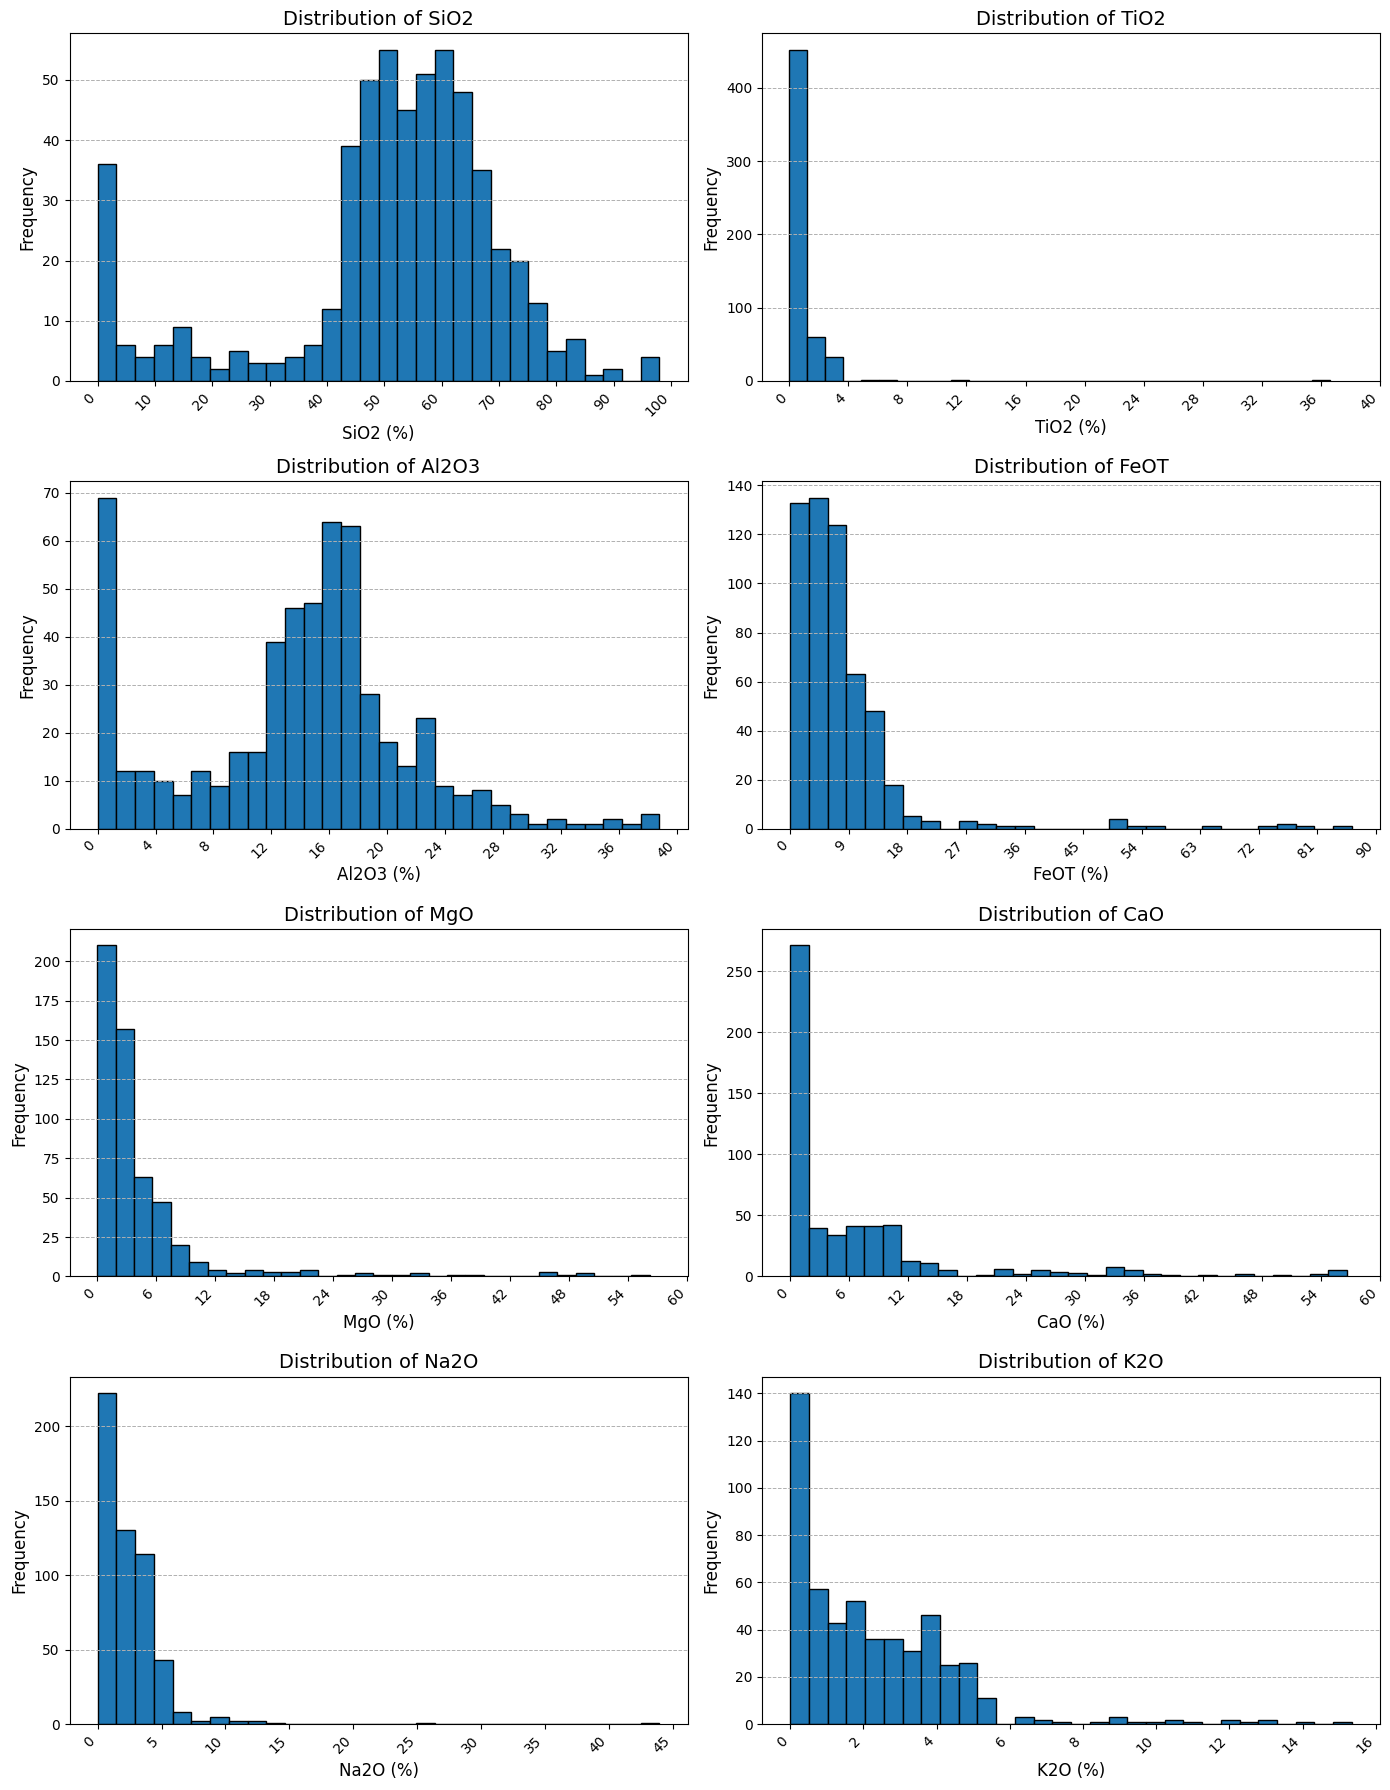
\includegraphics[width=\textwidth]{images/oxide_distributions.png}
    \caption{Distributions of various oxide concentrations in the dataset. The histograms show the frequency of concentration values for \ce{SiO2}, \ce{TiO2}, \ce{Al2O3}, \ce{FeO_T}, \ce{MgO}, \ce{CaO}, \ce{Na2O}, and \ce{K2O}.}
    \label{fig:oxide_distributions}
\end{figure*}

Figure~\ref{fig:oxide_distributions} illustrates the distributions of various oxide concentrations in our dataset.
Across all oxides, there is a general pattern of skewed distributions, with concentrations heavily weighted towards lower values.
This is particularly notable in \ce{TiO2}, \ce{FeO_T}, \ce{MgO}, \ce{CaO}, and \ce{Na2O}.
\ce{SiO2} and \ce{Al2O3} show more variability, with \ce{SiO2} exhibiting a bimodal distribution.
These distributions confirm the presence of extreme values across all oxides, which are significantly overrepresented or underrepresented, further complicating the model training process.

This necessitates careful dataset partitioning to ensure that the model training process accounts for these challenges, improving the generalizability and robustness of the models.

\subsubsection{Dataset Partitioning}\label{subsubsec:dataset_partitioning}
To ensure rigorous evaluation of our models and to address the challenges of data leakage and uneven distribution of extreme values, we have implemented a customized k-fold data partitioning procedure. 
This approach divides the dataset into $k$ folds, which it uses to define cross-validation data sets, as well as a training set and a test set.
The procedure ensures that all data points from a given target are only present in one of the $k$ folds, overcoming the challenge of data leakage we mention above.
Additionally, it ensures that extreme values are handled by redistributing them evenly across the training folds, preventing any single fold from being disproportionately influenced by these values.

\begin{algorithm}
\caption{Data Partitioning With Extreme Value Handling}
\label{alg:custom_kfold_cv}
\begin{algorithmic}[1]
\Require Dataset $\mathbf{D}$, group column $g$, target column $t$, number of splits $k$, percentile $p$, random seed $\textit{seed}$
\Ensure Training and validation sets for cross-validation $\mathbf{T}_\text{cv}$, training set $\mathbf{D}_\text{train}$, and test set $\mathbf{D}_\text{test}$
\State \label{line:seed} Set random seed for reproducibility if $\text{seed}$ is not None
\State \label{line:remove_duplicates} Remove duplicate entries based on $g$ and sort by $t$
\State \label{line:assign_folds} Assign fold numbers sequentially from 0 to $k-1$ to unique targets
\If{extreme values handling is enabled}
    \State \label{line:identify_extremes} Identify extreme values at percentiles $p$ and $1-p$
    \State \label{line:reassign_extremes} Reassign extreme values to folds $0$ to $k-2$
\EndIf
\State \label{line:merge_folds} Merge fold assignments information into the original dataset
\State \label{line:split_dataset} Split dataset into test set $\mathbf{D}_\text{test}$ (fold $k-1$) and remaining data $\mathbf{D}_\text{train}$
\State \label{line:create_folds} Create $k-1$ training and validation sets
\For{each fold $i$ from 0 to $k-2$}
    \State $\mathbf{T}_\text{train}[i] \gets \mathbf{D}_\text{train} \setminus \text{fold}_i$
    \State $\mathbf{T}_\text{val}[i] \gets \text{fold}_i$
    \State Append $(\mathbf{T}_\text{train}[i], \mathbf{T}_\text{val}[i])$ to $\mathbf{T}_\text{cv}$
\EndFor
\State \label{line:remove_fold_column} Remove fold column from all datasets
\State \Return $\mathbf{T}_\text{cv}, \mathbf{D}_\text{train}, \mathbf{D}_\text{test}$
\end{algorithmic}
\end{algorithm}

The procedure outlined in Algorithm~\ref{alg:custom_kfold_cv} begins by setting a random seed for reproducibility if one is provided (Line~\ref{line:seed}).
This ensures that the results are consistent across different runs of the algorithm.
Next, the dataset is processed to remove any duplicate entries based on the group column $g$ and then sorted by the target column $t$ (Line~\ref{line:remove_duplicates}).
This step ensures that each group is uniquely identified and ordered appropriately.
The dataset we illustrate in Table~\ref{tab:final_dataset_example} would require a group column $g$ of "\texttt{Target}" to group the data by target.
The target column $t$ refers to the column with the target variable, which would be the oxide for which we are predicting the concentration, for example, \ce{SiO_2}.
By sorting the dataset by the target column $t$, we ensure that the data is ordered by the target concentration values in ascending order.

Fold numbers are then assigned sequentially using a modulo operation to ensure a random-like distribution of the unique targets across the folds (Line~\ref{line:assign_folds}).
This means that, while the assignment process follows a sequence, the resulting distribution of targets is effectively randomized.
Fold numbers start in 0 and go up to $k-1$, as implied by the modulo operation.
If handling of extreme values is enabled, the algorithm identifies the top and bottom percentiles of the target values (Line~\ref{line:identify_extremes}).
These extreme values are then reassigned to the training folds (0 to \( k-2 \)), ensuring they are evenly distributed across these folds (Line~\ref{line:reassign_extremes}).

The fold assignments are then merged into the original dataset, as described in Line~\ref{line:merge_folds}.
Essentially, this step enables the partitioning steps that follow, by ensuring each data item has an associated fold number.
Following this, the dataset is divided into a test set, which always consists of the data points assigned to fold $k-1$, and the remaining data forms the training set, as outlined in Line~\ref{line:split_dataset}.
The training data is further divided into $k-1$ sets for cross-validation. 
For each fold $i$ where $i \in \{0, 1, \ldots, k-2\}$, we create a cross-validation training set $\mathbf{T}_\text{train}[i]$ by excluding the $i$-th fold from the set of $k-1$ folds, and use the $i$-th fold as the validation set $\mathbf{T}_\text{val}[i]$.
These pairs of training and validation sets are then appended to the list of cross-validation sets $\mathbf{T}_\text{cv}$ (Line~\ref{line:create_folds}).

Finally, the fold indicator column is removed from all datasets before returning the final partitions (Line~\ref{line:remove_fold_column}).
The fold indicator column was added to keep track of which data points belong to which folds, which is crucial for ensuring that data points are correctly partitioned into their respective training and test sets during cross-validation. 
This cleanup step ensures that the fold information does not interfere with subsequent data processing or model training.

The final output of this procedure consists of:
\begin{itemize}
    \item A set of tuples \(\mathbf{T}_\text{cv}\), where each tuple contains a training set and a validation set.
    \item The overall training set \(\mathbf{D}_\text{train}\), consisting of all the data points not in the test set.
    \item The test set \(\mathbf{D}_\text{test}\), distinct from the training set.
\end{itemize}

The data partitioning does not modify the original dataset; it merely partitions it.
For that reason, each of the datasets that are returned has the same structure as shown in Table~\ref{tab:final_dataset_example}.

Our method for handling extreme values ensures that the test set does not include samples outside the range seen in the training set.
This approach addresses several critical challenges and represents a deliberate trade-off to improve the reliability of our model evaluation:

Firstly, it mitigates the risk of uneven distribution of extreme values, which can disproportionately affect model performance metrics.
If extreme values are unevenly distributed between the training and test sets, the evaluation of the model can be heavily skewed, leading to unreliable and misleading performance metrics.
By redistributing extreme values evenly across the training folds, we ensure a more balanced and fair assessment of the model's capabilities during cross-validation.

Secondly, this trade-off allows for a more stable and reliable assessment of the model's performance on typical data points.
While the test set may be less representative of the full range of data, particularly regarding rare extreme values, the evaluation focuses on the model's ability to generalize from the training data to new data within the same distribution range.
This is prudent because, in many practical applications, the reliability of the model on typical data points is more critical than its performance on rare extremes.
By using cross-validation in conjunction with a separate test set, we ensure that the model is robust and performs well under typical conditions.

However, it is important to recognize the limitation this approach introduces: excluding extreme values from the test set means we can only confidently assess the model's performance within the range of the test set.
If we receive predictions outside this range, we cannot reliably assert their accuracy, as the model has not been fully evaluated on such data.
This could potentially make the model less useful in scenarios where predictions on extreme values are critical.
Nevertheless, cross-validation partially mitigates this issue by allowing the model to learn from extreme values during the training and validation phases, thereby improving its robustness.
Metrics obtained from cross-validation provide a broader picture of the model's accuracy and robustness across the entire dataset, including extreme values.

Therefore, although our approach may make the test set less representative of the full dataset, it is a deliberate trade-off aimed at achieving a more accurate and reliable evaluation of the model's generalization performance.

Our method is inspired by the approach described by \citet{andersonImprovedAccuracyQuantitative2017}.
They employed a similar strategy to assess the performance of their PLS model, using k-fold cross-validation and a separate test set.
Their process involved dividing the full set of laboratory data into five folds, using four for cross-validation and combining them as the final training set, while the fifth fold served as a test set.
For consistency, we also use $k = 5$ for our data partitioning.
Given that the $k$-th fold is used as the test set, having $k=5$ results in 4 folds for cross-validation.

Additionally, by using $k = 5$ folds, we have effectively chosen an 80\%/20\% split between the training and testing datasets.
In our experience, this ratio maximizes the training set's capacity for effective model learning while ensuring that the testing set is sufficiently representative to provide an accurate assessment of the model's performance on new data.
Allocating too much data to the testing set could compromise the comprehensiveness of the training set, undermining the model's ability to generalize effectively due to the limited availability of data.

\subsubsection{Cross-Validation}
% Section on cross validation approach
\subsection{Model and Preprocessing Selection}

Choosing the right models and preprocessing techniques for \gls{libs} data analysis is a challenging task. 
As the literature highlighted in Section~\ref{sec:related-work} suggests, a variety of models and preprocessing techniques promise to be adept at handling data that exhibit high-dimensionality, multi-collinearity, and matrix effects.
The literature also indicates that different machine learning models perform better on some oxides than others.
These challenges and model-specific strengths suggests that an optimal approach would involve combining multiple models. 
This notion is supported by the advent of models such as the \gls{moc}~\cite{cleggRecalibrationMarsScience2017} model, which combines the predictions of multiple models using a predetermined weighting for each model's predictions on a per-oxide basis.
While this approach improved accuracy compared to individual models, it required manual tuning of the weights for each model.
This manual tuning presents limitations, including the analysis required to determine appropriate weights and the risk of suboptimal weighting.
Given these limitations, it is reasonable to explore techniques that can automate the weighting process while still leveraging the strengths of multiple models.
To fulfill these criteria, we chose to adopt a stacking ensemble approach. 
Stacking, as described in Section~\ref{subsec:stacked-generalization}, is a method that utilizes multiple base estimators trained on the same data, whose predictions are then used to train a meta-learner.
By combining a diverse set of base models, stacking can correct for the biases of individual models.
Since each model focuses on different patterns within the data, stacking mitigates the inherent biases of individual models by estimating and correcting for these biases.
This approach of leveraging the strength of multiple models that each model the problem differently can lead to better generalization on unseen data by automating and potentially improving upon manual tuning through the use of a meta-learner to discern patterns in the base predictors' outputs. \cite{wolpertstacked_1992, survey_of_ensemble_learning}
However, some consideration has be made towards training of the base models in order to prevent data leakage and overfitting.
As emphasized by \citet{cvstacking}, if the base models are trained on the same dataset, the meta learner might favor certain base models over others.
This can cause the meta learner to be influenced by the same patterns and biases that the base models are susceptible to, leading to overfitting.
To mitigate this risk and ensure generalizability, a cross-validation strategy should be employed to ensure that the meta learner's training data accurately reflects the true performance of the base learners.

We adopted an experimental approach to empirically evaluate the potential of various models and preprocessing techniques, to be used in our stacking ensemble, ensuring that our selections were informed by our literature review while also allowing for independent assessment and validation.

We had several considerations to guide our selection of preprocessing techniques.
Firstly, our review of the literature revealed that there seems to be no consensus on a single, most effective normalization method for \gls{libs} data.
Therefore, we included traditional normalization methods in our experiments, such as z-score normalization, Min-Max scaling, and Max Absolute scaling.
This approach allowed us to determine which normalization method was most effective for our dataset. 
Additionally, dimensionality reduction techniques are considered by the literature to be effective techniques for \gls{libs} data due to its high dimensionality. 
Specifically, \gls{pca} has been widely adopted by the spectroscopic community as an established dimensionality reduction technique~\cite{pca_review_paper}. 
However, \citet{pca_review_paper} make the case that the assumptions for \gls{pca} regarding linearity of the data are only met up to a certain point, after which it breaks. 
They argue that this non-linearity inherent in the data makes \gls{kernel-pca} a valid candidate for \gls{libs} data. 
Based on their review of the field, and our own review of the literature, not many have studied the effectiveness of \gls{kernel-pca} in the context of \gls{libs} data. 
Therefore, we decided to include this in our experiments to further assess its potential. 
In addition to the non-linearity, \citet{pca_review_paper} also argue that the assumptions of normality in the data are not always met in \gls{libs} data. 
For this reason, we decided to include power transformation and quantile transformation in our experiments, as models such as \gls{pca} benefit from a normal distribution of the data. 
We assume that models such as \gls{pls} may also benefit from a more Gaussian-like data distribution, given that the model is partly based on \gls{pca}.

While these preprocessing techniques are not an exhaustive list, they represent a diverse set of methods.
Techniques such as feature selection were not considered in this study to limit its scope and due to time constraints.

We also had several requirements for the model selection.
The selected models for experimentation had to be diverse to ensure sufficient breadth in our results, enabling informed decisions about which models to include in the final stacking ensemble pipeline.
Additionally, the models had to be suitable for regression tasks. 
In the absence of research specific to \gls{libs} data, we selected models that have shown promise in other domains.
Our literature review found that a variety of models fit this criteria.
For example, \citet{andersonPostlandingMajorElement2022} demonstrated that models such as \gls{gbr}, \gls{pls}, \gls{lasso}, and \gls{rf} were each effective at predicting different major oxides from \gls{libs} data. 
Additionally, \citet{svrforlibs} showed that \gls{svr} outperforms \gls{plsr} in predicting \ce{Si}, \ce{Ca}, \ce{Mg}, \ce{Fe}, and \ce{Al} using \gls{libs} data.
As a result, we included \gls{gbr}, \gls{pls}, \gls{lasso}, \gls{rf}, and \gls{svr} in our experiments.

In the neural network domain, \cite{ann_libs_soil_analysis} showed that on \gls{libs} data their 3-layer \gls{ann} relative error of prediction for \ce{Ca}, \ce{Fe}, \ce{Al} was below 20\%.
Likewise, \citet{yangConvolutionalNeuralNetwork2022} showed that \gls{cnn} outperformed methods such as \gls{logreg}, \gls{svm} and linear discriminant analysis at correctly classifying twelve different types of rocks based on \gls{libs} data. 
While this example for \gls{cnn} is a classification task, \gls{cnn} can be adjusted for regression tasks by changing the loss function and output layer.
Based on these factors, we decided to include \gls{ann} and \gls{cnn} in our experiments to further increase the diversity of our model selection.

To further bolster our selection pool, we chose to include models that were in the same family of models as those that showed promise in the literature.

\gls{xgboost} was included as an option based on its promising accuracy in various settings.
For example \citet{xgboost_in_biomedicie} showed that \gls{xgboost} outperformed models such as \gls{rf} and \gls{svm} in predicting biological activity based on quantitative description of the compound's molecular structure. 
Another example is \citet{xgboost_in_heart_disease} that used \gls{xgboost} to predict heart disease, where \gls{xgboost} outperformed \gls{rf} and \gls{etr} at correctly classifying patients with heart disease.
Due to these factors and the limited study of \gls{xgboost} in the context of \gls{libs} data, we decided to include it in our experiments.

Following the same logic, we included \gls{ngboost}. 
\gls{ngboost} is a recent model introduced by \citet{duan_ngboost_2020} that, according to their work, improves upon \gls{gbr} by using a more sophisticated loss function and a more advanced gradient boosting algorithm.
Limited research has been conducted using this algorithm in the context of \gls{libs} data. 
However, \citet{ngboost_landslide} showed that \gls{ngboost} outperformed \gls{xgboost} and \gls{rf} in correctly determining landslide-prone fields, with an AUC of 0.898 compared to 0.871 and 0.863 for \gls{xgboost} and \gls{rf}, respectively.

Finally, \gls{ridge}, \gls{enet}, \gls{etr}, and \gls{lasso} were included in various studies and showed promising results, even if they were not the top performers in their respective studies.
Therefore, we chose to include these in our experiments to further diversify our model selection. 

Table~\ref{tab:preprocessing-models} summarizes the preprocessing techniques and models selected for our experimentation.

\begin{table}[ht]
\centering
\begin{tabularx}{\columnwidth}{>{\raggedright\arraybackslash}X}
\toprule
\textbf{Normalization / Scaling:} \\
\midrule
Z-Score Normalization \\
Min-Max Normalization \\
Max Absolute Scaling \\
Robust Scaling \\
Norm 3 \\
\midrule
\textbf{Transformation Methods:} \\
\midrule
Power Transformation \\
Quantile Transformation \\
\midrule
\textbf{Dimensionality Reduction Methods:} \\
\midrule
PCA \\
Kernel PCA \\
\midrule
\textbf{Model Types:} \\
\midrule
\textbf{Regression Models:} \\
\quad Partial Least Squares \\
\quad Support Vector Regression \\
\quad Elastic Nets \\
\quad Least Absolute Shrinkage and Selection Operator \\
\quad Ridge Regression \\
\textbf{Ensemble Models:} \\
\quad Random Forest \\
\quad Gradient Boost Regression \\
\quad Extra Trees Regression \\
\quad XGBoost \\
\quad Natural Gradient Boosting \\
\textbf{Neural Networks:} \\
\quad Artificial Neural Networks \\
\quad Convolutional Neural Networks \\\bottomrule
\end{tabularx}
\caption{Overview of Preprocessing Techniques and Models}
\label{tab:preprocessing-models}
\end{table}
\section{Baseline \& Replica}\label{sec:baseline_replica}
For analyzing Martian geological samples, the \gls{chemcam} team currently uses the \gls{moc} model~\cite{cleggRecalibrationMarsScience2017}.
This model integrates \gls{pls} and \gls{ica} to predict the composition of major oxides.

As shown in figure \ref{fig:moc_pipeline}, the input to the \gls{moc} model is the \gls{ccs} data, mentioned in Section~\ref{sec:problem_definition}.
This spectral data is collected on Earth in a laboratory setting simulating the Martian environment.
The instrument used to collect this data is a \gls{libs} instrument replicating the \gls{chemcam} instrument on the Curiosity rover.
Both the \gls{chemcam} and laboratory instrument consist of three spectrometers, each producing 2048 channels.
These spectrometers are used to capture the \gls{uv}, \gls{vio}, and \gls{vnir} regions of the spectrum.
For each sample, five \gls{ccs} datasets are collected by firing 50 laser shots at five different locations on the sample and processing the raw spectral readings \cite{wiensPreflightCalibrationInitial2013}.
Consequently, the \gls{ccs} data for each sample forms a high-dimensional Intensity Tensor $I$\ref{matrix:intensity} with dimensions $5 \times 50 \times 6144$.
An entry in this matrix represents the intensity of a specific wavelength in nanometers.
Complementing the data is the matrix of the corresponding major oxide concentrations for each sample $C$\ref{matrix:concentration}, which serves as the target variable for the model.
For more details, refer to Section 5 in \citet{p9_paper}.

The \gls{pls} and \gls{ica} phases of the \gls{moc} operate in parallel, and their predictions are blended to form the final predictions.
Though the \gls{moc} model has proven useful, it suffers from limitations in predictive accuracy and robustness.
An overview of the \gls{moc} model is shown in Figure~\ref{fig:moc_pipeline}.

\begin{figure}
	\centering
	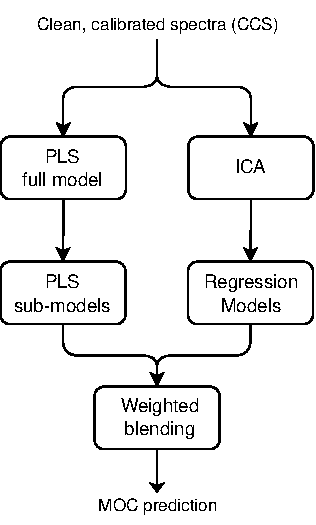
\includegraphics[width=0.225\textwidth]{images/moc_pipeline.pdf}
	\caption{Overview of the \gls{moc} model.}
	\label{fig:moc_pipeline}
\end{figure}

In \citet{p9_paper}, we presented our efforts to replicate the \gls{moc} model.
Based on the insights gained from that work, we have made several modifications to the replica in preparation for this work.

Our replica only utilized a single dataset for the \gls{ica} phase, while the original model used all five datasets.
This difference was due to the original paper not specifying how the five datasets were used, and so we designed an experiment to determine how to use them in a way that would most closely replicate the original model.
We initially assumed that the datasets were aggregated and used as a single dataset.
This approach, however, did not align with the original model's results, likely due to the loss of information from the individual datasets.
Following this discovery, we modified the replica to instead use the datasets in the same way as in the \gls{pls1-sm} phase, which yielded results aligning more closely with the original model.

Furthermore, our initial replica used a random train/test split for training, in contrast to the original model's manual curation to ensure representation of extreme compositions in both sets.
This difference stemmed from the original authors' application of domain expertize in their dataset curation --- a process we could not directly replicate.
Nevertheless, we found that automatically identifying extreme compositions and ensuring that they were present in both the training and testing sets brought us closer to the original model.
We chose to pull out the $n$ largest and smallest samples by concentration range, for each oxide, and reserve them for the training set.
Then we would do a random split on the remaining dataset, such that the final train/test split would be a $80\%/20\%$ split.

With these changes, we created a more accurate replica of the \gls{moc} model, which we will use as our baseline for the rest of this paper.
We have presented these changes to one of the original authors of~\citet{cleggRecalibrationMarsScience2017}, who confirmed that they were reasonable and in line with the original model's implementation.

Table~\ref{tab:replica_results_rmses} shows the \gls{rmse}s of the original models and our replicas after the changes.
Figure~\ref{fig:rmse_histograms} illustrates the distribution of these \gls{rmse}s as a grouped histogram.
The results show that the \gls{rmse}s of our replicas exhibit similar tendencies to the original models.
However, in some cases, our replicas have a lower \gls{rmse} than the original models, and in others, they have a higher \gls{rmse}.
These differences are due to a number of factors.

Firstly, the original models were trained with datasets from 1600mm and 3000mm standoff distances~\cite{cleggRecalibrationMarsScience2017}, while we only had access to the 1600mm dataset for our replicas.
Additionally, we automated the outlier removal for the PLS1-SM phase, unlike the original manual process.
As mentioned, the original authors manually curated their training and test sets, ensuring a broad elemental range, while we implemented an automatic process for our replicas due to lack of domain expertise.
Differences might also stem from varied implementation specifics, such as programming languages and libraries used.

\begin{table*}
	\centering
	\begin{tabular*}{\textwidth}{@{\extracolsep{\fill}}lllllll}
		\hline
		Element    & \gls{pls1-sm} (original) & PLS1-SM (replica) & \gls{ica} (original) & ICA (replica) & \gls{moc} (original) & \gls{moc} (replica) \\
		\hline
		\ce{SiO2}  & 4.33                     & 4.52              & 8.31                 & 8.63          & 5.30                 & 5.61                \\
		\ce{TiO2}  & 0.94                     & 0.49              & 1.44                 & 0.54          & 1.03                 & 0.61                \\
		\ce{Al2O3} & 2.85                     & 1.79              & 4.77                 & 3.18          & 3.47                 & 2.47                \\
		\ce{FeO_T} & 2.01                     & 2.16              & 5.17                 & 2.87          & 2.31                 & 1.82                \\
		\ce{MgO}   & 1.06                     & 0.91              & 4.08                 & 3.11          & 2.21                 & 1.56                \\
		\ce{CaO}   & 2.65                     & 1.73              & 3.07                 & 3.28          & 2.72                 & 2.09                \\
		\ce{Na2O}  & 0.62                     & 0.80              & 2.29                 & 1.39          & 0.62                 & 1.33                \\
		\ce{K2O}   & 0.72                     & 0.72              & 0.98                 & 1.38          & 0.82                 & 1.91                \\
		\hline
	\end{tabular*}
	\caption{\gls{rmse}s of the original and our replicas of the \gls{pls1-sm}, \gls{ica}, and \gls{moc} models.}
	\label{tab:replica_results_rmses}
\end{table*}

\begin{figure*}
	\centering
	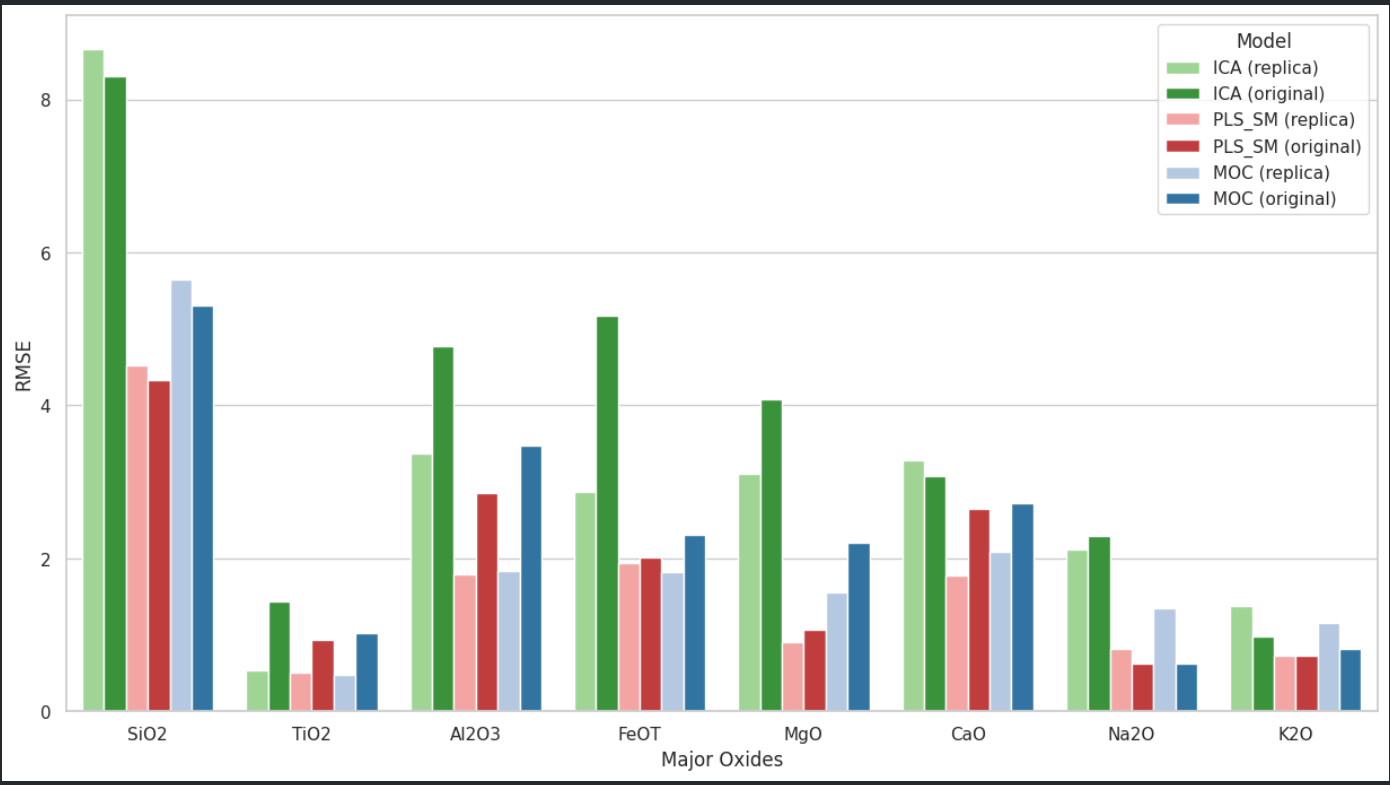
\includegraphics[width=0.85\textwidth]{images/rmse_historgram.png}
	\caption{Grouped histogram of the \gls{rmse}s of the original and our replicas of the \gls{pls1-sm}, \gls{ica}, and \gls{moc} models.}
	\label{fig:rmse_histograms}
\end{figure*}

Through a series of comparative experiments, we showed that the model selection was the primary cause of these limitations, and we showed how both \gls{ann} and \gls{gbr} methods could be used to improve the model's predictive accuracy and robustness.
This is further underscored by work from the SuperCam team.
In 2021, the Perseverance rover landed on Mars, equipped with the SuperCam instrument, which is the successor to the \gls{chemcam} instrument.
As part of the ongoing work to support the SuperCam instrument, \citet{andersonPostlandingMajorElement2022} experimented with various machine learning models to predict the composition of major oxides in geological samples using the SuperCam \gls{libs} calibration dataset.
While the team decided to retain \gls{pls} for analyzing certain oxides, \gls{ica} was entirely discontinued.
Instead, models based on \gls{gbr}, \gls{rf}, and \gls{lasso} were selected for other oxides.
This decision reinforces our finding that \gls{ica} regression models fall short in accurately predicting the composition of major oxides in geological samples.
Consistent with our observations, \gls{gbr} was also identified as a high-performing model in their analyses.

\section{Methodology}\label{sec:methodology}
As part of our goal to evaluate the performance of each of the components in the pipeline, the first step was to create a replica of the original pipeline described by \citet{cleggRecalibrationMarsScience2017}
Since we did not have access to the original source code implementing the pipeline, we have replicated it at accurately as we could based on the available information.
We have had to make some assumptions due to insufficient information regarding some components, which we detail in this section.
In addition, some aspects of the pipeline rely on qualitative assessments made by the original authors --- something we cannot do because we are not domain experts.
Consequently, our pipeline is not identical to the original, but we have strived to make it as close as possible while favoring conservative choices and omitting implementations where information about the original pipeline was unclear.
This decision was driven by the aspiration to ensure that the baseline results remained minimally influenced by our methodological choices.

This section is dedicated to describing the methodology of our pipeline, how it differs from the original, and which design choices we have made and why.
Furthermore, we delve into the experiments we have conducted to evaluate the performance of our pipeline such that we can identify the components that contribute the most to the overall error.

Section \ref{sec:methodology_pls1}, we focus on the specifics of the PLS1-SM phase, detailing its associated data preprocessing procedures.
In Section \ref{sec:methodology_ica} then details the ICA phase, including its unique data preprocessing steps.
Lastly, Section \ref{sec:methodology_moc} presents a description of the MOC phase of the pipeline.

\subsection{PLS1-SM}\label{sec:methodology_pls1}
The PLS1-SM phase in our pipeline largely follows the same approach as described in \citet{andersonImprovedAccuracyQuantitative2017} with a few exceptions.
We detail our approach and the differences from the original pipeline in this section.

\subsubsection{Data Preprocessing}\label{sec:pls1_data_preprocessing}
The preprocessing of the data is illustrated in Figure~\ref{fig:pls_data_preprocessing}.

\begin{figure}
	\centering
	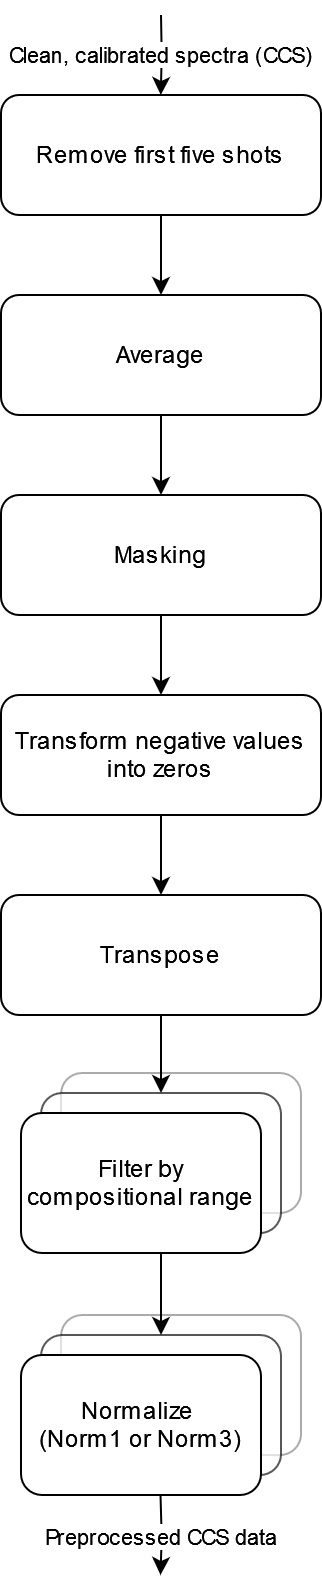
\includegraphics[width=0.175\textwidth]{images/pls_preprocessing.png}
	\caption{The PLS1-SM data preprocessing phase in our recreation of the pipeline. The filtering and normalization steps are done independently for each oxide.}
	\label{fig:pls_data_preprocessing}
\end{figure}
\noindent
We start by removing the first five shots from the data similarly to \citet{cleggRecalibrationMarsScience2017} since they are typically contaminated by dust that covers the target before being removed by the laser-produced shock waves.
Then the remaining 45 shots from each location are averaged, resulting in a single spectrum per location with a total of five spectra per target.
As mentioned in Section~\ref{sec:data_overview}, the edges of the spectral regions contain noise, so we apply masking to the data to remove these regions.
The masked regions, which do not contain unique major element diagnostic peaks, are excluded to enhance the accuracy and reliability of the quantitative analysis\cite{cleggRecalibrationMarsScience2017}.
The dataframe is then transformed through a transpose operation, swapping the rows and columns.
This gives us a dataframe with the average intensities per sample as rows, and the wavelengths as columns.
All negative values are then transformed into zeros since negative values are not physically possible.
Given the pre-defined compositional ranges for each oxide in \citet{andersonImprovedAccuracyQuantitative2017}, we filter out wavelengths outside of these ranges.
The range is defined by an upper and a lower bound, and any wavelength outside of this range is removed.
Finally, we apply two different normalization techniques, Norm1 and Norm3, to the data.
This results in two separate datasets, each normalized in a distinct manner but derived from the same original dataset.
ICA and PLS-SM are then performed on each of these datasets separately.
The reason for this is that, as \citet{cleggRecalibrationMarsScience2017} found, some of the oxides are better modeled with data normalized using Norm1, while others are better modeled with data normalized using Norm3.

\subsubsection{PLS1-SM Regression}\label{sec:methodology_pls1-sm_regression}
The PLS phase of the pipeline follows a submodel approach to make wt. \% predictions for each oxide, as previously mentioned in Section~\ref{sec:introduction}.

%TODO add information about the hyperparameters used
The training of the models follows the same approach as described in \citet{andersonImprovedAccuracyQuantitative2017} and is illustrated in Figure~\ref{fig:pls_training}.
However, assumptions have been made regarding the k-fold cross-validation process, as the authors are ambiguous in their description of the number of folds used.
We interpreted their description as using a 20\% holdout split and a 4-fold on the remaining 80\% of the data --- resulting in a total of 5 folds.
Furthermore, we have decided to automate outlier removal as described in Section~\ref{sec:methodology_outlier_removal} rather than performing it manually.
Finally, similar hyperparameters have been used for the PLS models as described in \citet{andersonImprovedAccuracyQuantitative2017}.

\begin{figure}
	\centering
	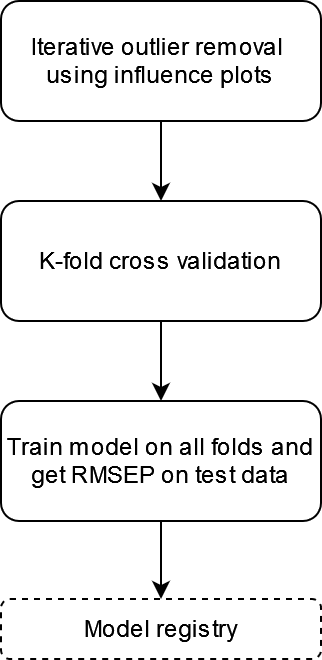
\includegraphics[width=0.175\textwidth]{images/pls_training.png}
	\caption{The PLS1-SM training phase in our recreation of the pipeline. This phase is repeated for each oxide's compositional range.}
	\label{fig:pls_training}
\end{figure}

Obtaining predictions for each of the eight oxides, for a single spectrum, requires a separate predictions for each oxide. While PLS regression is capable of multivariate regression, each oxide calls for different hyperparameter configurations and normalization procedures.
The submodels for an oxide generally include a full model, a low, mid, and high model. They are named after the compositional range in the data they are trained on. Here, compositional range refers to the known compositional values for a sample, which we use to filter the sample data to include samples data within that range.
These compositional ranges overlap, which creates a blending range.
Some oxides have only two compositional ranges, which means the model may have low-high as a blending range.

As mentioned, the PLS submodels approach is repeated for each oxide and is illustrated in Figure~\ref{fig:pls_inference}.
Given some new data sample, the full model gives an initial compositional prediction for its oxide.
Based on this prediction, the data is then "binned" into one of five concentration ranges -- the three submodel ranges and two blending ranges.
For each of these five concentration ranges, there is one or two corresponding \textit{submodel(s)}.
These submodels are used to make predictions in the corresponding concentration range after the full model has made its initial predictions.
The submodels are specialized in either low, low-mid, mid, mid-high, high concentration ranges, which are defined in Table 2 in \citet{andersonImprovedAccuracyQuantitative2017}.
If the full model predicts a concentration that falls within a blending range, the approach described in Section~\ref{sec:pls_submodels} is used to combine the predictions from the corresponding submodels.

\begin{figure}
	\centering
	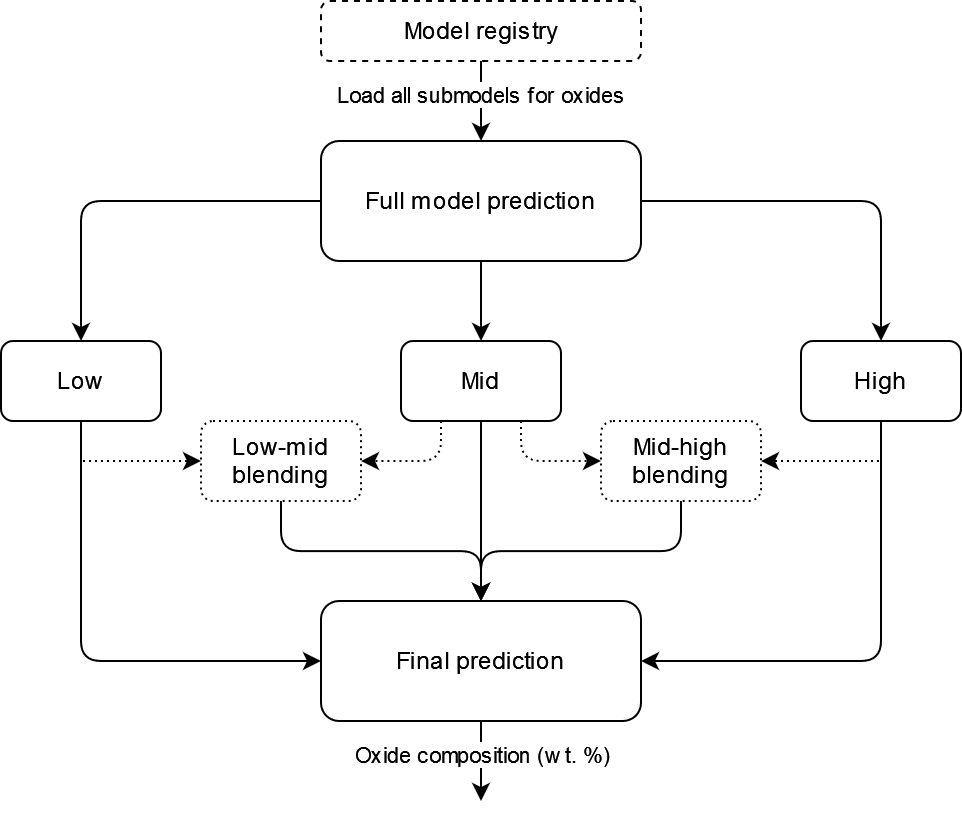
\includegraphics[width=0.45\textwidth]{images/pls_inference.png}
	\caption{The PLS1-SM inference phase in our recreation of the pipeline.}
	\label{fig:pls_inference}
\end{figure}

\subsubsection{Outlier Removal with Mahalanobis Distance and Chi-Squared Test}\label{sec:methodology_outlier_removal}
As mentioned in section \ref{sec:outlier_removal}, if the Mahalanobis distances can be shown to follow a chi-squared distribution, then the chi-squared test can be used to determine whether a sample is an outlier.
Since we do not have the expertise to make a qualitative assessment of the outliers, we have instead decided to use this property of the Mahalanobis distances to automatically detect outliers.
This works by computing the Mahalanobis distance for each data point in the training set, followed by a comparison of these distances against a chi-squared distribution.
A data point is classified as an outlier if its Mahalanobis distance corresponds to a chi-squared statistic that exceeds the critical value of the chi-squared distribution, which is determined by the specified degrees of freedom $\nu$.
The critical value is determined by the significance level $\alpha$ and $\nu$.
Since we have leverage and spectral residuals as our two dimensions, we have $\nu = 2$, because the number of dimensions is equal to the number of degrees of freedom\cite{aggarwal_outlier_2017}.

The outlier removal process is done iteratively because of the phenomenon described in \citet{cleggRecalibrationMarsScience2017} where removing outliers can cause new outliers to appear.
The process is as follows:
\begin{enumerate}
    \item Compute the Mahalanobis distances for each sample in the training set.
    \item Determine chi-squared statistics for these distances.
    \item Eliminate outliers exceeding the chi-squared critical value.
    \item Train a new model on the remaining samples.
    \item Repeat until model no longer improves as measured by the RMSE.
\end{enumerate}

It should be noted that our outlier removal process is conservative to avoid removing too many samples and as such, we have set our significance level $\alpha$ to 0.975.
This means that we are willing to accept a 2.5\% chance of falsely removing a sample that is not an outlier.

\subsection{ICA}\label{sec:methodology_ica}
The ICA phase in our pipeline can be seen in figure \ref{fig:ica_phase}.
In this section, we delve into the differences between our pipeline and the original, and we discuss the rationale behind our choices.

\begin{figure}
	\centering
	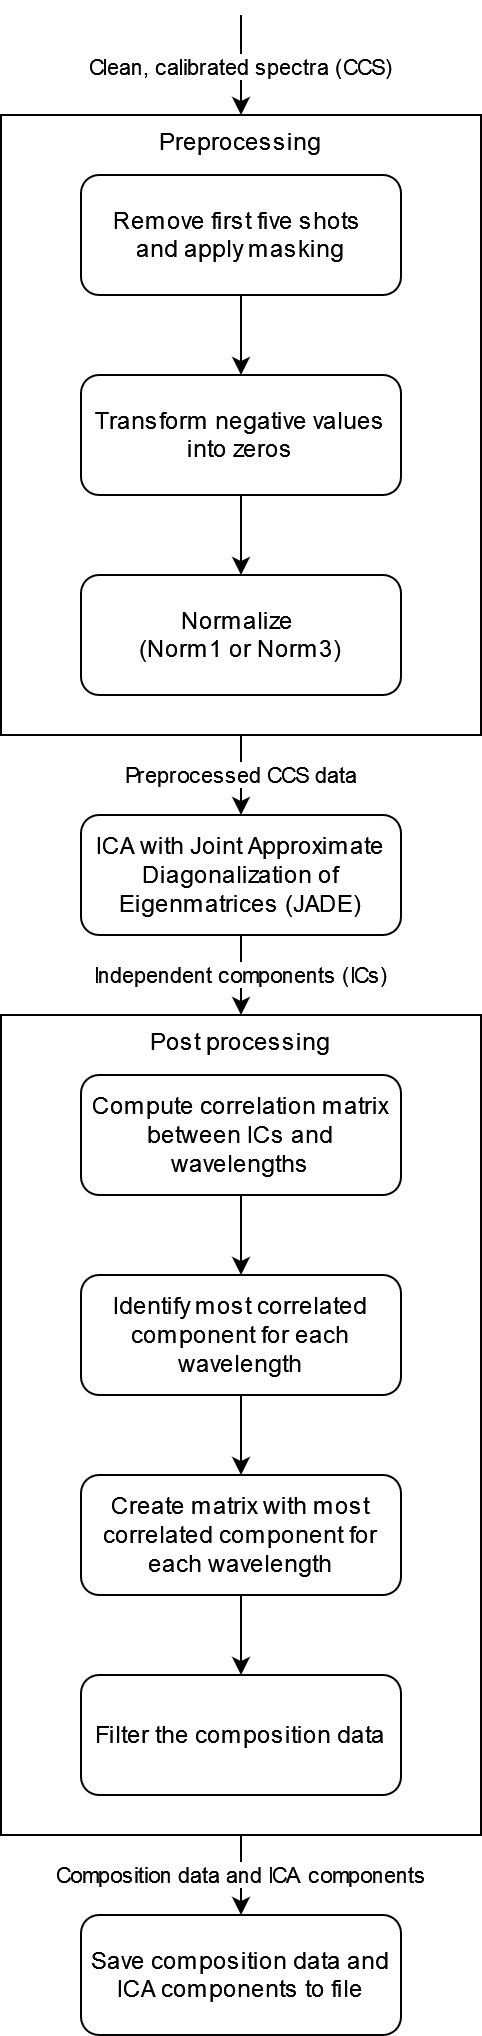
\includegraphics[width=0.2675\textwidth]{images/ica_phase.png}
	\caption{The ICA phase in our recreation of the pipeline.}
	\label{fig:ica_phase}
\end{figure}

\subsubsection{Data Preprocessing}\label{sec:ica_data_preprocessing}
For ICA, the first five shots are removed from the data.
We then apply masking to the data to remove the same regions as in the PLS1-SM phase.
Afterwards, we transform all negative values into zeros.
Then we normalize the data using Norm1 and Norm3.

In contrast to \citet{cleggRecalibrationMarsScience2017} however, we do not weigh by the inverse of the instrument response function (IRF) before normalizing.
The purpose of the IRF is to calibrate the measured signal to physical units since different pixels have different sensitivities\cite{wiensChemcam2012}.
One argument for inverting the IRF is that it introduces more noise in areas of interest on the spectrum by multiplying with a high value as part of the conversion to physical units.
However, during a conversation with one of the original authors of \citet{cleggRecalibrationMarsScience2017}, criticism was raised against this.
Specifically, the author pointed out that weighing by the inverse of the discards the alignment between the spectral data collected by the instrument in Los Alamos and the spectral data collected by the instrument on Mars.
If the same instrument were used for all analyses, one could argue that the IRF (apart from the inverse square law correction) part is irrelevant, but that is not the case here; there are two different instruments --- one in Los Alamos and one on Mars.
Based on these considerations, we have decided to not weigh by the inverse of the IRF.

In addition, because \citet{cleggRecalibrationMarsScience2017} does not mention how each of the five location datasets are used for each sample, we have decided to only use one for each sample.
This likely does not produce as accurate results as using all five location datasets would, since we do not get a full representation of the sample that was shot at by the laser, instead only getting a partial representation from a single location.
Nevertheless, to avoid deviating significantly from \citet{cleggRecalibrationMarsScience2017}'s methodology or making unfounded assumptions about their data processing, we have opted for this more conservative approach.
Our goal is to test each of the components of the pipeline individually rather than trying to reproduce the results to absolute perfection.

Similarly, in our replica of the pipeline, we have not incorporated outlier detection in the ICA part of the pipeline primarily because \citet{cleggRecalibrationMarsScience2017} does not describe their implementation sufficiently enough for replication without unsubstantiated assumptions.
They mention the use of Median Absolute Deviation for this purpose, but the specifics of their approach remain unclear.
Our decision to omit outlier detection in the ICA phase of our pipeline is also influenced by a preference for retaining a more comprehensive dataset, despite the potential inclusion of outliers.
Further supporting this decision is input from one of the original authors involved in the ChemCam project.
This author highlighted the extensive efforts invested in developing the ChemCam calibration dataset, suggesting a low presence of significant outliers.
While it would be ideal to include outlier detection in the ICA phase to ensure alignment with the original pipeline, implementing it based on substantial assumptions would be counterproductive, potentially compromising the integrity of our analysis.

After examining the results in section \ref{sec:results}, we will discuss the implications of these design choices in section \ref{sec:discussion}.

\subsubsection{Joint Approximate Diagonalization of Eigenmatrices (JADE) and Regression}
After preprocessing the data, we are ready to perform ICA.
This is done using the Joint Approximate Diagonalization of Eigenmatrices (JADE) algorithm, which is used to calculate the mixing matrix.
This mixing matrix is an $N \times M$ matrix, where $N$ is the number of samples and $M$ is the number of independent components.
By taking the product of the mixing matrix and the normalized data, we get the estimated sources.
This new matrix is an $M \times P$ matrix, where $M$ is the number of independent components, and $P$ is the number of wavelengths.

After performing ICA, we post-process by computing the correlation between the independent components and the wavelengths.
Using this, we can identify which wavelengths are associated with which independent components by computing the maximum correlation for each wavelength.
This gives us a matrix of ICA scores that we then use for regression.

\begin{figure}
	\centering
	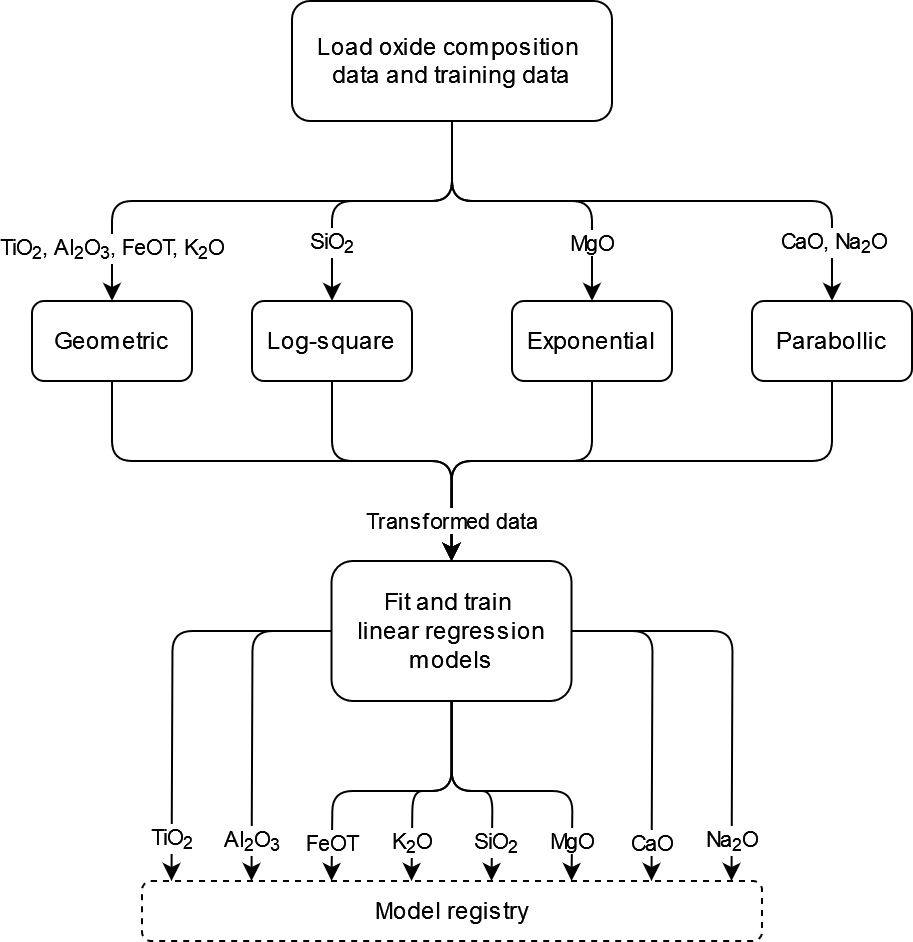
\includegraphics[width=0.45\textwidth]{images/ica_regression.png}
	\caption{Regression in the ICA phase of our recreation of the pipeline.}
	\label{fig:ica_regression}
\end{figure}

The regression process is illustrated in figure \ref{fig:ica_regression}.
\citet{cleggRecalibrationMarsScience2017} perform four more types of regression in addition to linear regression, namely parabolic, exponential, geometric and logsquare.
For each oxide, they used the type of regression and normalization that produced the best results.

We use Linear Regression for all oxides and instead transform the data to fit the model similar to \citet{kuo_detecting_2018}.
Initially, it might appear limiting, but by applying transformations to the features --— for example by taking logs, square roots, etc. --- it's possible to achieve an almost linear relationship with the target variable.

% TODO: Move this table to the results section and embed our own results in it as well to show the baseline results compared to the original results.
% This can be seen in table \ref{tab:regression_types}, which is taken from \citet{cleggRecalibrationMarsScience2017}.

% \begin{table}[h]
% \centering
% \begin{tabular*}{\columnwidth}{@{\extracolsep{\fill}}lccc}
% \toprule

% Element & Norm & Law type    & RMS \\ \midrule
% Si      & 1    & Logsqaure   & 6.7 \\
% Ti      & 3    & Geometric   & 0.6 \\
% Al      & 3    & Geometric   & 4.4 \\
% Fe      & 1    & Geometric   & 2.2 \\
% Mg      & 1    & Exponential & 3.0 \\
% Ca      & 1    & Parabolic   & 1.0 \\
% Na      & 3    & Parabolic   & 0.6 \\
% K       & 3    & Geometric   & 0.4 \\
% \bottomrule
% \end{tabular*}
% \caption{The summary of each ICA model characteristics from \citet{cleggRecalibrationMarsScience2017}.}
% \label{tab:regression_types}
% \end{table}

\subsection{MOC}\label{sec:methodology_moc}
As described in section \ref{sec:moc_derivation}, the result of the PLS1-SM and ICA are combined to produce the final MOC model, which weights the results of the two techniques in favor of the one that performs best for each oxide.
The specific weights used for each oxide can be seen in table \ref{tab:weighted_sum_oxide}.
Note that the weights for Ti, Mg and Ca have been set to 50/50 since \citet{cleggRecalibrationMarsScience2017} does not mention the weights they used for these elements.

\begin{table}[h]
\centering
\begin{tabular*}{\columnwidth}{@{\extracolsep{\fill}}lcc}
\toprule
Element  & PLS1-SM (\%) & ICA (\%) \\ \midrule
Al       & 75           & 25      \\
Fe       & 75           & 25      \\
Si       & 50           & 50      \\
Na       & 40           & 60      \\
K2       & 25           & 75      \\
Ti*      & 50           & 50      \\
Mg*      & 50           & 50      \\
Ca*      & 50           & 50      \\
\bottomrule
\end{tabular*}
\caption{Weighted Sum of Oxide Percentages. Elements marked with an asterisk (*) have been set to 50/50 as they are unspecified in \citet{cleggRecalibrationMarsScience2017}}
\label{tab:weighted_sum_oxide}
\end{table}

\subsection{Experiments}\label{sec:methodology_experiments}
To evaluate the performance of each of the components in the pipeline, we focus our experiments on three main aspects:

\begin{itemize}
	\item \textbf{Outlier removal} to assess the impact of leaving outliers in the dataset or using a different outlier removal method.
	\item \textbf{Hyperparameter tuning} to assess the impact of different hyperparameter configurations.
	\item \textbf{Other models} to compare the performance of the PLS1-SM and ICA models to other models.
\end{itemize}

\noindent
Given that the original authors did not perform experiments using alternative methods to demonstrate the efficacy of their chosen approach, this omission results in a lack of comprehensive understanding regarding the full potential of the pipeline's performance.
While they did perform hyperparameter tuning, they did not conduct experiments using different outlier removal methods or alternative models.
This raises questions about the optimality of the chosen methodology, as a comparative analysis with different methodologies could reveal superior approaches.
Experimenting with alternative methods means that we can uncover which components contribute the most to the overall error and therefore would benefit the most from further research and development.
Should a substitution of a component within the pipeline with an alternative method yield improved outcomes, it would indicate that the currently employed method represents a limitation in the overall pipeline, thus highlighting an area that necessitates enhancement.

\subsubsection{Experiment: Outlier Removal}\label{sec:experiment_outlier_removal}
The original PLS1-SM identified outliers manually by inspecting the leverage and spectral residuals plots.
We have instead chosen to automate this based on the reasons described in Section~\ref{sec:methodology_outlier_removal}.
It would therefore be intriguing to examine the impact on the pipeline's performance when this process is adjusted.
Firstly, examining the performance implications of completely omitting outlier removal would be worthwhile.
This experiment is justified given the substantial efforts dedicated to developing the ChemCam calibration dataset as mentioned in Section~\ref{sec:ica_data_preprocessing}, which implies a minimal presence of significant outliers.
Furthermore, experimenting with various significance levels for the chi-squared test could reveal whether a more or less conservative approach is advantageous.

In the ICA phase, the original authors employed the Median Absolute Deviation (MAD) for outlier removal, yet the detailed methodology of their approach was not fully delineated.
Consequently, in our version of the pipeline, we chose to exclude the outlier removal step during the ICA phase to avoid introducing unsubstantiated assumptions, as described in Section~\ref{sec:ica_data_preprocessing}.
This decision allows us to evaluate the intrinsic effectiveness of the ICA phase without the influence of outlier removal.
Introducing outlier removal using MAD in our replication of the pipeline presents an opportunity to assess its impact on the pipeline's efficacy.
By comparing the results with and without MAD, we can quantitatively measure the utility of this step.
Such an experiment is crucial for understanding whether MAD significantly contributes to reducing noise and improving data quality, thereby enhancing the overall performance of the machine learning pipeline.
This experiment would also offer insights into the robustness of the ICA phase against outliers, providing a more comprehensive understanding of the pipeline's capabilities and limitations.

\subsubsection{Experiment: Hyperparameter Tuning}\label{sec:experiment_hyperparameter_tuning}
\citet{cleggRecalibrationMarsScience2017} use qualitative judgement to identify hyperparameters for their PLS1-SM model.
This approach carries a risk of inaccuracies without sufficient domain expertise, given the challenges in guaranteeing the optimality of chosen hyperparameters.
Lacking such expertise, we opted for a more systematic and automated methodology to determine hyperparameters for our PLS1-SM model.

Similarly, the authors use eight independent components for their ICA algorithm, but do not provide any experimental results justifying that this is the optimal number of components.
As such, it is possible that the performance of the ICA phase could be improved by experimenting with a variety of components.

For the PLS1-SM model we decided to use the common grid search algorithm for testing different hyperparameters for the PLS models.
% Explain set up...

Since each independent component does not necessarily correlate one-to-one with the number of elements that one wishes to identify in a spectra, we decided to experiment with a number of components ranging between 4 and 25.
This range is within the vicinity of the original selection of components whilst providing us with a set of reasonable extremes.

% Probably show the setup in some way

\subsubsection{Experiment: Other Models}\label{sec:experiment_other_models}
\citet{cleggRecalibrationMarsScience2017} have only compared their new approach with the original method presented by \citet{wiensPreFlight3}, and have not conducted experiments using alternative methods to establish the superiority of their chosen approach.
Therefore, we decided to compare the performance of the PLS1-SM and ICA models to other models.
The objective is to evaluate two distinct scenarios. In the first scenario, we aim to conduct a direct comparison between the MOC model and an alternative model. The second scenario revolves around substituting either PLS or ICA with a different model and then calculating a weighted average.
We have decided to conduct the experiments using the following models:

\begin{itemize}
	\item \textbf{XGBoost}, a gradient boosting algorithm, \cite{chen_xgboost_2016}.
	\item \textbf{ANN}, a neural network model, \cite{scikit-learn}.
	% More? Random Forest, SVM, etc.
\end{itemize}

\section{Experimental Design}\label{sec:methodology}
This section outlines the experimental design used to identify the top-$n$ models to be used in our stacking ensemble.
We first describe the prequisite data preparation for all our experiments, followed by a description of the hardware and software used.
Next, we outline the design of our initial experiment, aimed at providing a preliminary assesment of the models selected in Section~\ref{sec:model_selection}.
Following this, we present and discuss the results of this experiment.
We then describe the design of our main experiment, where we use our hyperparameter tuning framework to identify the top-$n$ models.
Finally, we present and discuss the results of this experiment.

\subsection{Data Preparation}\label{sec:data-preparation}
The first step in our methodology is to prepare the datasets for model training and evaluation.
As mentioned in Section~\ref{sec:data-overview}, the data used in this study was obtained from \gls{nasa}'s \gls{pds} and consists of \gls{ccs} data and major oxide compositions for various samples.

The initial five shots from each sample are excluded because they are usually contaminated by dust covering the sample, which is cleared away by the shock waves produced by the laser \cite{cleggRecalibrationMarsScience2017}.
The remaining 45 shots from each location are then averaged, yielding a single spectrum $s$ per location $l$ in the \texttt{Averaged Intensity Tensor} (Tensor \ref{matrix:averaged_intensity}), resulting in a total of five spectra for each sample.

At this stage, the data still contains noise at the edges of the spectrometers.
These edges correspond to the boundaries of the three spectrometers, which collectively cover the \gls{uv}, \gls{vio}, and \gls{vnir} light spectra.
The noisy edge ranges are as follows: 240.811-246.635 nm, 338.457-340.797 nm, 382.138-387.859 nm, 473.184-492.427 nm, and 849-905.574 nm.
In addition to being noisy regions, these regions do not contain any useful information related to each of the major oxides.
Consequently, these regions are masked by zeroing out the values, rather than removing them, as they represent meaningful variation in the data~\cite{cleggRecalibrationMarsScience2017}.

Additionally, as a result of the aforementioned preprocessing applied to the raw \gls{libs} data, negative values are present in the \gls{ccs} data.
These negative values are not physically meaningful, since you cannot have negative light intensity \cite{p9_paper}.
Similar to the noisy edges, these negative values are also masked by zeroing out the values.

We transpose the data so that each row represents a location and each column represents a wavelength feature.
Each location is now represented as a vector of wavelengths, with the corresponding average intensity values for each wavelength.
These vectors are then concatenated to form a tensor, giving us the full \texttt{Averaged Intensity Tensor}.

For each sample, we have a corresponding set of major oxide compositions in weight percentage (wt\%).
These compositions are used as the target labels for the machine learning models.
An excerpt of this data is shown in Table \ref{tab:composition_data_example}.
While the \textit{Target}, \textit{Spectrum Name}, and \textit{Sample Names} are part of the dataset, our analysis focuses primarily on the \textit{Sample Names}.
The concentrations of the eight oxides \ce{SiO2}, \ce{TiO2}, \ce{Al2O3}, \ce{FeO_T}, \ce{MnO}, \ce{MgO}, \ce{CaO}, \ce{Na2O}, and \ce{K2O} represent the expected values for these oxides in the sample, serving as our ground truth. The \textit{MOC total} is not utilized in this study.

\begin{table*}
\centering
\caption{Excerpt from the composition dataset (from \citet{p9_paper}).}
\begin{tabular}{lllllllllllll}
\toprule
     Target & Spectrum Name & Sample Name & \ce{SiO2} & \ce{TiO2} & \ce{Al2O3} & \ce{FeO_T} & \ce{MnO} & \ce{MgO} & \ce{CaO} & \ce{Na2O} & \ce{K2O} & \ce{MOC total} \\
\midrule
AGV2 & AGV2 & AGV2 & 59.3 & 1.05 & 16.91 & 6.02 & 0.099 & 1.79 & 5.2 & 4.19 & 2.88 & 97.44 \\
BCR-2 & BCR2 & BCR2 & 54.1 & 2.26 & 13.5 & 12.42 & 0.2 & 3.59 & 7.12 & 3.16 & 1.79 & 98.14 \\
$\vdots$ & $\vdots$ & $\vdots$ & $\vdots$ & $\vdots$ & $\vdots$ & $\vdots$ & $\vdots$ & $\vdots$ & $\vdots$ & $\vdots$ & $\vdots$ & $\vdots$ \\
TB & --- & --- & 60.23 & 0.93 & 20.64 & 11.6387 & 0.052 & 1.93 & 0.000031 & 1.32 & 3.87 & 100.610731 \\
    TB2 & --- & --- & 60.4 & 0.93 & 20.5 & 11.6536 & 0.047 & 1.86 & 0.2 & 1.29 & 3.86 & 100.7406 \\
\bottomrule
\end{tabular}
\label{tab:composition_data_example}
\end{table*}

The major oxide weight percentages are appended to the matrix of spectral data, forming the final dataset.
This dataset is shown in Table~\ref{tab:final_dataset_example}.
The \textit{Target} column corresponds to the sample name, while the \textit{ID} column contains the unique identifier for each location.

\begin{table*}
\centering
\caption{Excerpt from the final dataset (values have been rounded to two decimal places for brevity).}
\footnotesize
\begin{tabular}{llllllllllllllllllllll}
\toprule
    240.81   & $\cdots$     & 425.82    & 425.87   & $\cdots$ & 905.57  & \ce{SiO2} & \ce{TiO2} & \ce{Al2O3} & \ce{FeO_T} & \ce{MgO} & \ce{CaO} & \ce{Na2O} & \ce{K2O} & Target     & ID \\
\midrule
	0        & $\cdots$     & 1.53e+10 & 1.62e+10 & $\cdots$ & 0        & 56.13     & 0.69 & 17.69 & 5.86 & 3.85 & 7.07 & 3.32 & 1.44 & jsc1421     & jsc1421\_2013\_09\_12\_211002\_ccs \\
	0        & $\cdots$     & 1.28e+10 & 1.30e+10 & $\cdots$ & 0        & 56.13     & 0.69 & 17.69 & 5.86 & 3.85 & 7.07 & 3.32 & 1.44 & jsc1421     & jsc1421\_2013\_09\_12\_211143\_ccs \\
    0        & $\cdots$     & 1.87e+10 & 1.83e+10 & $\cdots$ & 0        & 56.13     & 0.69 & 17.69 & 5.86 & 3.85 & 7.07 & 3.32 & 1.44 & jsc1421     & jsc1421\_2013\_09\_12\_210628\_ccs \\
    0        & $\cdots$     & 1.77e+10 & 1.78e+10 & $\cdots$ & 0        & 56.13     & 0.69 & 17.69 & 5.86 & 3.85 & 7.07 & 3.32 & 1.44 & jsc1421     & jsc1421\_2013\_09\_12\_210415\_ccs \\
    0        & $\cdots$     & 1.75e+10 & 1.79e+10 & $\cdots$ & 0        & 56.13     & 0.69 & 17.69 & 5.86 & 3.85 & 7.07 & 3.32 & 1.44 & jsc1421     & jsc1421\_2013\_09\_12\_210811\_ccs \\
    0        & $\cdots$     & 5.52e+10 & 3.74e+10 & $\cdots$ & 0        & 57.60     & 0.78 & 26.60 & 2.73 & 0.70 & 0.01 & 0.38 & 7.10 & pg7         & pg7\_2013\_11\_07\_161903\_ccs \\
    0        & $\cdots$     & 5.09e+10 & 3.41e+10 & $\cdots$ & 0        & 57.60     & 0.78 & 26.60 & 2.73 & 0.70 & 0.01 & 0.38 & 7.10 & pg7         & pg7\_2013\_11\_07\_162038\_ccs \\
    0        & $\cdots$     & 5.99e+10 & 3.97e+10 & $\cdots$ & 0        & 57.60     & 0.78 & 26.60 & 2.73 & 0.70 & 0.01 & 0.38 & 7.10 & pg7         & pg7\_2013\_11\_07\_161422\_ccs \\
    0        & $\cdots$     & 5.22e+10 & 3.47e+10 & $\cdots$ & 0        & 57.60     & 0.78 & 26.60 & 2.73 & 0.70 & 0.01 & 0.38 & 7.10 & pg7         & pg7\_2013\_11\_07\_161735\_ccs \\
    0        & $\cdots$     & 5.29e+10 & 3.62e+10 & $\cdots$ & 0        & 57.60     & 0.78 & 26.60 & 2.73 & 0.70 & 0.01 & 0.38 & 7.10 & pg7         & pg7\_2013\_11\_07\_161552\_ccs \\
	$\vdots$ & $\cdots$ & $\vdots$ & $\vdots$ & $\cdots$ & $\vdots$ & $\vdots$ & $\vdots$ & $\vdots$ & $\vdots$ & $\vdots$ & $\vdots$ & $\vdots$ & $\vdots$ & $\vdots$ & $\vdots$ \\
\midrule
\end{tabular}
\label{tab:final_dataset_example}
\end{table*}
\subsection{Experimental Setup}
Experiments were conducted on a machine equipped with an Intel Xeon Gold 6242 CPU, featuring 16 cores and 32 threads.
The CPU has a base clock speed of 2.80 GHz and a maximum turbo frequency of 3.90 GHz.
The system has 64 GB of RAM and runs on Ubuntu 22.04.2 LTS.
Models were implemented using Python 3.10.11.
The primary libraries used were Scikit-learn 1.4.2, XGBoost 2.0.3, Torch 2.2.2, NumPy 1.26.4, Pandas 2.2.1, Keras 3.2.1 and Optuna 3.6.1.
Additionally, all experiments were run using the hyperparameter optimization tool described in Section~\ref{subsec:hyperparameter_tuning_tool}. % TODO: Add correct ref once other PR is in
\subsection{Design for Initial Experiment}\label{sec:initial-experiment}
As described in Section~\ref{sec:proposed_approach}, we conducted a series of initial experiments to evaluate the performance of various machine learning models on the prediction of major oxide compositions from our \gls{libs} dataset.
These experiments aimed to provide a preliminary assessment of the models' performance, allowing us to identify the most promising models for further evaluation and inclusion in our stacking ensemble.
All models were trained on the same preprocessed data using the Norm 3 preprocessing method described in Section~\ref{sec:norm3}.
This ensured that the models' performance could be evaluated under consistent and comparable conditions.

All models were trained using our data partitioning and cross-validation strategy, as described in Section~\ref{subsec:validation_testing_procedures}. 
To ensure as fair of a comparison between models as possible, all models were trained using as many default hyperparameters as possible, and those hyperparameters that did not have default options were selected based on values found in the literature.
However, due to the nature of the neural network models' architecture, some extra time was spent on tuning the models to ensure a fair comparison.
This included using batch normalization for the \gls{cnn} model, as early assesments showed that this was necessary to produce reasonable results.
Finally, we evaluated each model once per oxide given the selected configuration of hyperparameters. 
As stated, the goal of this experiment was merely to get an initial indication of the performance of the models.

The hyperparameters used for the models in the initial experiment can be found in the Appendix~\ref{subsec:initial_experiment_hyperparameters}.
\section{Results}
We present the results of our experiments in this section.

\subsection{Visual and Statistical Analysis of \ce{SiO_2} Distribution in Partitioned Data}\label{sec:visual_analysis}
This section provides a detailed visualization and statistical analysis of the \ce{SiO_2} concentration distribution across data partitions, following the customized k-fold data partitioning procedure described in Section~\ref{subsec:validation_testing_procedures}.
We perform this analysis to validate the consistency of our data partitioning method and to provide a visual understanding of the data distribution it creates.
The analysis focuses on \ce{SiO_2} as a representative example.
We have conducted similar analyses for other oxides, but they are omitted here for brevity.

Figures \ref{fig:histogram_grid_plot} and \ref{fig:histogram_kde_plot} illustrate the histograms and \gls{kde} curves for \ce{SiO_2} concentrations in each training fold, the test set, and their combined distributions.
The consistent histograms and \gls{kde} curves across different training folds indicate that the data distribution within each fold closely matches the overall distribution, confirming their consistency and representativeness.

Figure \ref{fig:original_and_post_fold_plot} contrasts the \ce{SiO_2} concentration distribution before and after data partitioning.
The left plot shows the original distribution, while the right plot displays the fold-assigned distribution, color-coded by fold.
This visualization highlights that the partitioning strategy maintains the overall data distribution while ensuring balanced representation across folds.

\begin{figure*}[h!]
    \centering
    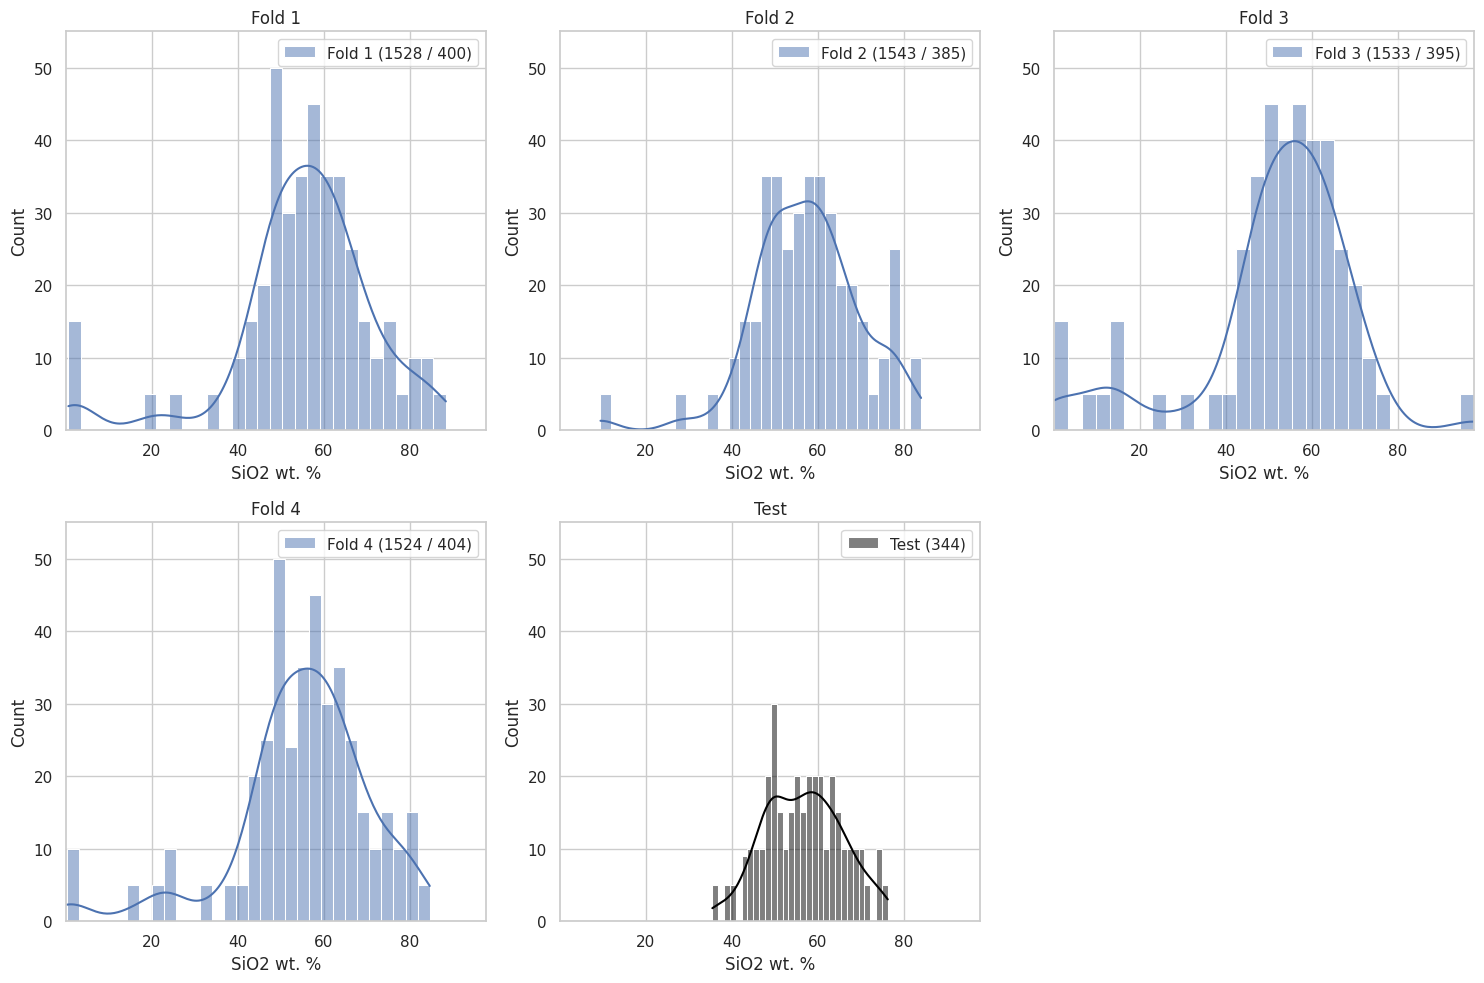
\includegraphics[width=\textwidth]{images/histogram_grid_plot.png}
    \caption{Histogram and \gls{kde} of \ce{SiO_2} Distribution in Each Fold. The y-axis represents the count of samples per bin, and the x-axis represents \ce{SiO_2} concentration. The notation in the legend indicates the amount of instances in the training/validation sets.}
    \label{fig:histogram_grid_plot}
\end{figure*}

\begin{figure*}[h!]
    \centering
    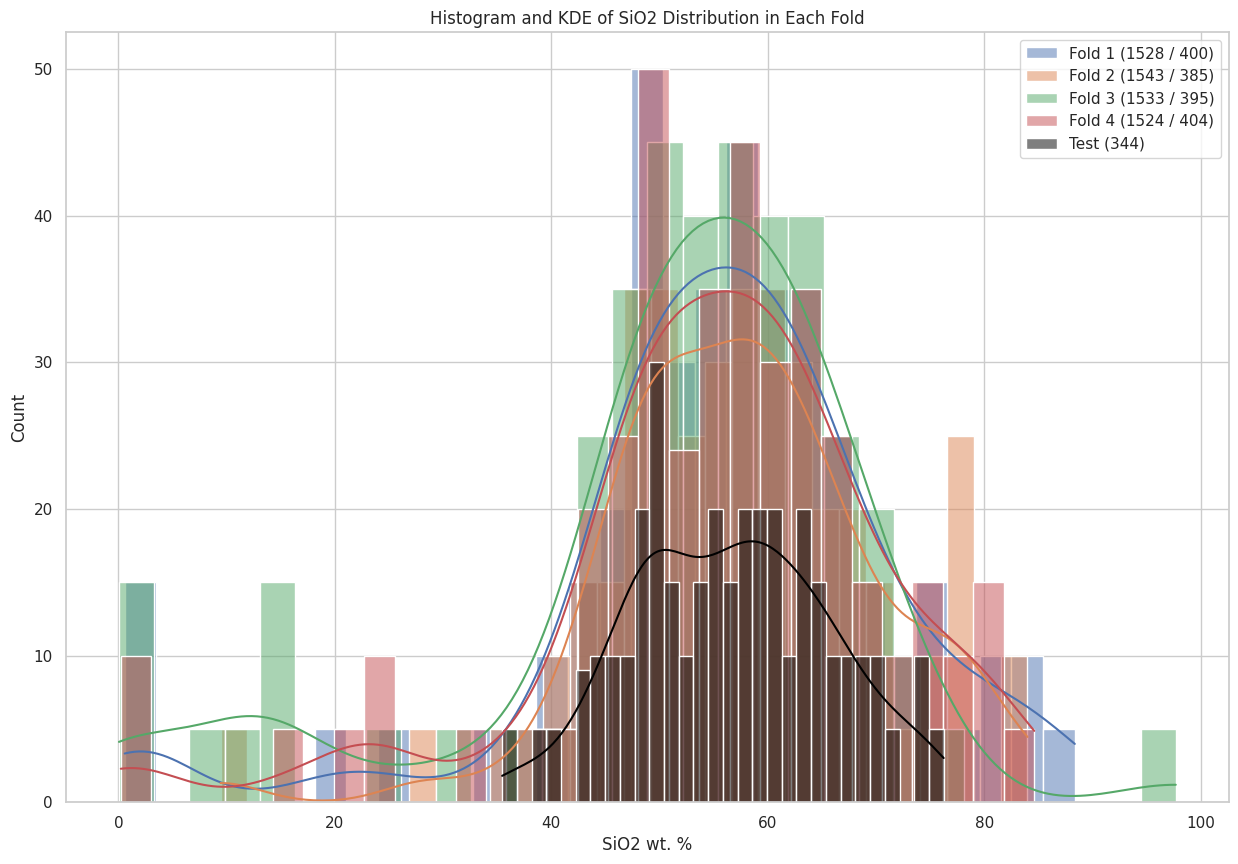
\includegraphics[width=\textwidth]{images/histogram_kde_plot.png}
    \caption{Combined Histogram and \gls{kde} of \ce{SiO_2} Distribution in Each Fold. The y-axis represents the count of samples per bin, and the x-axis represents \ce{SiO_2} concentration. The notation in the legend indicates the amount of instances in the training/validation sets.}
    \label{fig:histogram_kde_plot}
\end{figure*}

\begin{figure*}[h!]
    \centering
    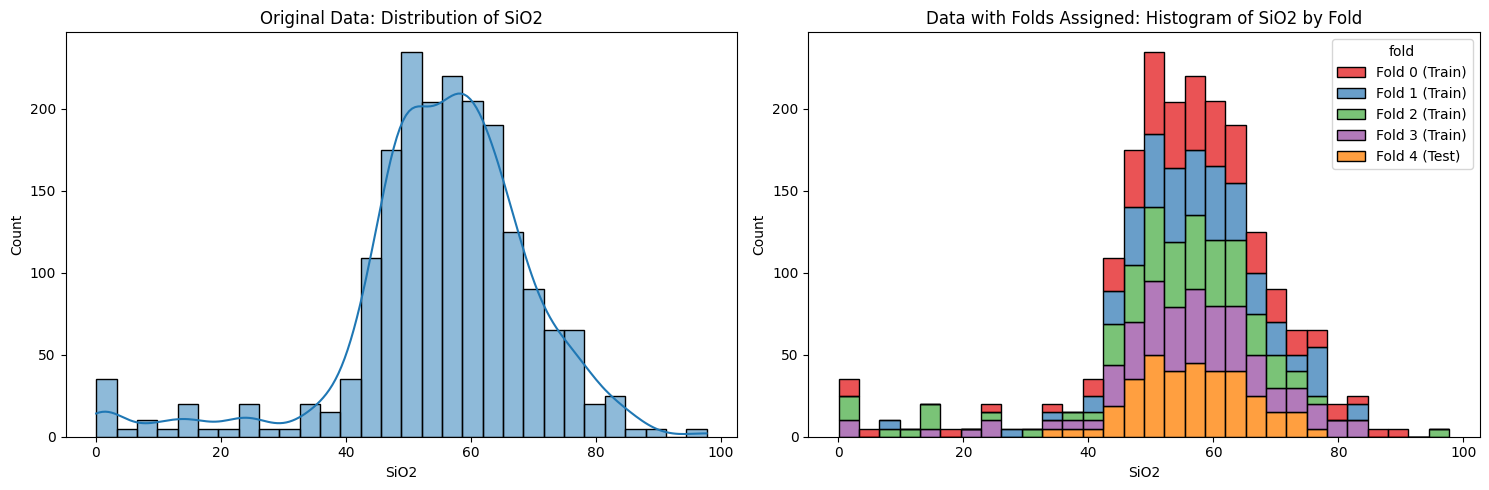
\includegraphics[width=\textwidth]{images/original_and_post_fold.png}
    \caption{Distribution of \ce{SiO_2} concentrations before and after fold assignment. The left plot shows the original distribution of \ce{SiO_2}, while the right plot shows the distribution with folds assigned, color-coded to indicate the different folds.}
    \label{fig:original_and_post_fold_plot}
\end{figure*}


To further validate our visual analysis, we can look at quantitative measures such as the means and standard deviations of \ce{SiO_2} concentrations across the folds and the overall dataset.

\begin{figure*}[htbp]
    \centering
    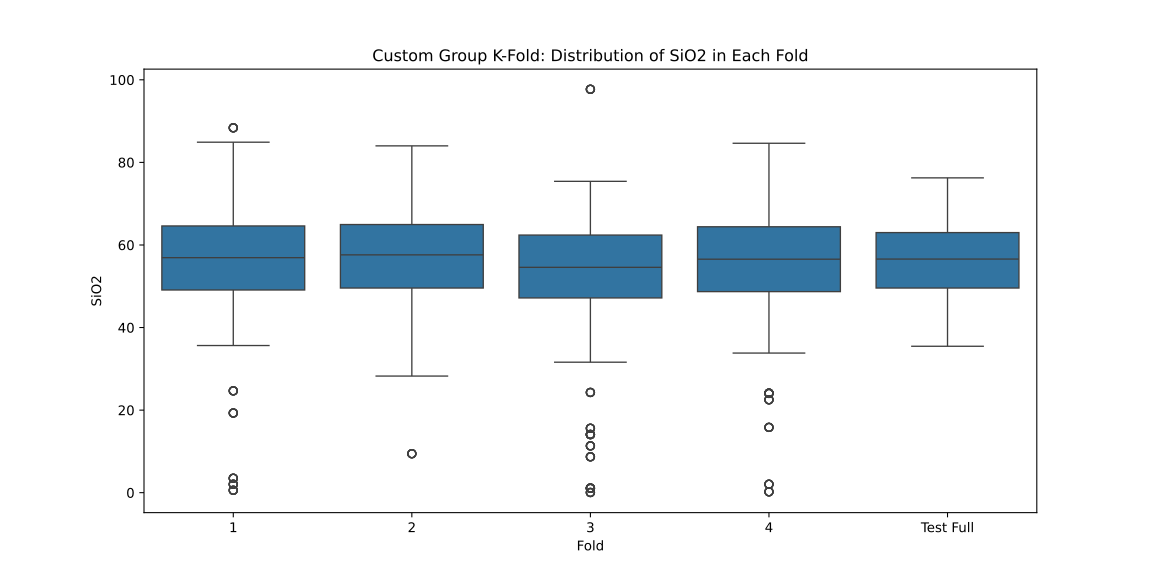
\includegraphics[width=\textwidth]{images/distribution_plot.png}
    \caption{Distribution of \ce{SiO_2} concentrations across cross-validation folds, training set, test set, and the entire dataset. The mean and standard deviation statistics for each partition are indicated figure.}
    \label{fig:siO2_distribution}
\end{figure*}

From Figure~\ref{fig:siO2_distribution}, it is evident that the means and standard deviations of \ce{SiO_2} concentrations for each fold, as well as the combined training set, are consistent with those of the full dataset.
This quantitative consistency supports the visual evidence that each training fold is representative of the entire dataset.
Furthermore, we can see that the standard deviation in the training sets is higher than the standard deviation in the test set, which is expected given the reassignment of extreme values to the training sets.

In conclusion, the visual and statistical analyses presented in this section confirm that our customized k-fold data partitioning procedure effectively maintains balanced and representative distributions across all folds.
This consistency is crucial for the robustness and generalizability of our models, as discussed in Section~\ref{subsec:validation_testing_procedures}.
The alignment between the visual evidence and the quantitative measures reinforces the reliability of our approach, ensuring that our models are well-equipped to perform accurately on unseen data.


% \subsection{Data Analysis}
% Description of the samples used and their relevance.
% Explain how and why these samples were chosen.

% \section{Methodology}
% \section{Baseline}
In \citet{p9_paper}, we presented our efforts to replicate the MOC model by \citet{cleggRecalibrationMarsScience2017}.
This effort was motivated by our desire to understand the model and its performance better, and to experiment with its components to determine how it could be improved.
However, as discussed, there were some differences between our replica and the original model.
These differences were caused by missing information in the original paper, and so rather than introducing our own assumptions, we designed experiments to determine the best way to replicate the model.

initially, our replication omitted the use of the \gls{mad} for outlier removal in the data preprocessing stage, a step included in the original model.
The omission was due to the lack of information regarding its implementation within the processing pipeline.
To rectify this, we experimented with applying \gls{mad} at various stages in the pipeline.
We determined that its application post-removal of the initial five shots, and prior to masking and normalization, most closely mirrored the outcomes of the original model.

Furthermore, our replica only utilized a single dataset for the \gls{ica} phase, while the original model used all five datasets.
This difference was due to the original paper not specifying how the five datasets were used, and so we designed an experiment to determine how to use them in a way that would most closely replicate the original model.
We initially assumed that the datasets were aggregated and used as a single dataset.
This approach, however, did not align with the original model's results, likely due to the loss of information from the individual datasets.
Following this discovery, we instead used the datasets in the same way as we did in the \gls{pls1-sm} phase, which yielded results aligning more closely with the original model.

Finally, our original replica used a random train/test split for training, in contrast to the original model's manual curation to ensure representation of extreme compositions in both sets.
This difference stemmed from the original authors' application of domain expertize in their dataset curation --- a process we could not directly replicate.
Nevertheless, we found that automatically identifying extreme compositions and ensuring that they were present in both the training and testing sets brought us closer to the original model.

With these changes, we have created a more accurate replica of the \gls{moc} model, which we will use as our baseline for the rest of the paper.
As an additional measure, we have presented these changes to one of the original authors, who confirmed that they were reasonable and in line with the original model's implementation.

Table \ref{tab:replica_results_rmses} shows the \gls{rmse}s of the original models and our replicas after these changes.
Figure~\ref{fig:rmse_histograms} illustrates the distribution of these \gls{rmse}s as a grouped histogram.

\begin{table*}
\centering
\begin{tabular*}{\textwidth}{@{\extracolsep{\fill}}lllllll}
\hline
Element    & \gls{pls1-sm} (original) & PLS1-SM (replica) & \gls{ica} (original) & ICA (replica) & \gls{moc} (original) & \gls{moc} (replica) \\
\hline
\ce{SiO2}  & 4.33                     & 4.52              & 8.31                 & 8.66          & 5.30                 & 5.64                \\
\ce{TiO2}  & 0.94                     & 0.50              & 1.44                 & 0.54          & 1.03                 & 0.48                \\
\ce{Al2O3} & 2.85                     & 1.80              & 4.77                 & 3.37          & 3.47                 & 1.84                \\
\ce{FeO_T} & 2.01                     & 1.94              & 5.17                 & 2.87          & 2.31                 & 1.82                \\
\ce{MgO}   & 1.06                     & 0.91              & 4.08                 & 3.01          & 2.21                 & 1.56                \\
\ce{CaO}   & 2.65                     & 1.77              & 3.07                 & 3.28          & 2.72                 & 2.09                \\
\ce{Na2O}  & 0.62                     & 0.82              & 2.29                 & 2.11          & 0.62                 & 1.34                \\
\ce{K2O}   & 0.72                     & 0.73              & 0.98                 & 1.37          & 0.82                 & 1.16                \\
\hline
\end{tabular*}
\caption{\gls{rmse} of the original and our replicas of the \gls{pls1-sm}, \gls{ica}, and \gls{moc} models.}
\label{tab:replica_results_rmses}
\end{table*}

\begin{figure*}[ht]
	\centering
	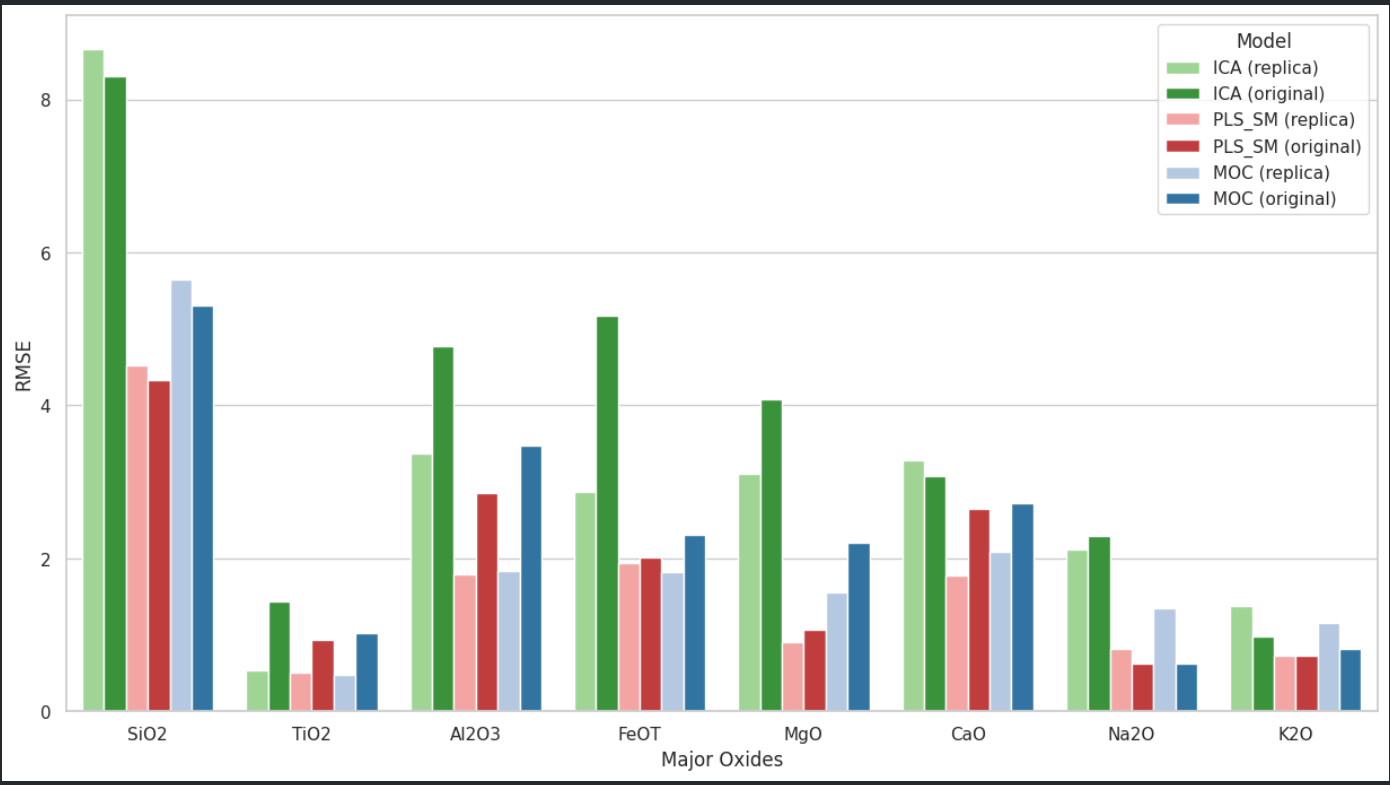
\includegraphics[width=0.85\textwidth]{images/rmse_historgram.png}
	\caption{Grouped histogram of the \gls{rmse}s of the original and our replicas of the \gls{pls1-sm}, \gls{ica}, and \gls{moc} models.}
	\label{fig:rmse_histograms}
\end{figure*}


\section{Conclusion}
Conclusion (the story again, in short, emphasizing the results)

Summary of the main findings of the report.
Reiteration of the significance of the established benchmarks to the subsequent part of the project.

\section{Recommendations for Future Work}
Suggestions for potential improvements or modifications in the methodology.
Identification of any additional benchmarks that may be relevant for future studies.
